% !Mode:: "TeX:UTF-8"
% !TEX program = xelatex

\def\usewhat{xelatex}                               
\documentclass[12pt,openany,oneside]{ctexbook}
                                                     % 本科生毕业论文通常采用单页排版
% !Mode:: "TeX:UTF-8"
%  Authors: 张井   Jing Zhang: prayever@gmail.com     天津大学2010级管理与经济学部信息管理与信息系统专业硕士生
%           余蓝涛 Lantao Yu: lantaoyu1991@gmail.com  天津大学2008级精密仪器与光电子工程学院测控技术与仪器专业本科生

%%%%%%%%%% Package %%%%%%%%%%%%
\usepackage{CJK}
\usepackage{lmodern}
\usepackage[T1]{fontenc}
\usepackage{graphicx}                       % 支持插图处理
\usepackage[a4paper,text={146.4true mm,239.2 true mm},top= 26.2true mm,left=31.8 true mm,head=6true mm,headsep=6.5true mm,foot=16.5true mm]{geometry}
                                            % 支持版面尺寸设置
\usepackage[squaren]{SIunits}               % 支持国际标准单位

\usepackage{titlesec}                       % 控制标题的宏包
\usepackage{titletoc}                       % 控制目录的宏包
\usepackage{fancyhdr}                       % fancyhdr宏包 支持页眉和页脚的相关定义
%\usepackage{ctex}                     % 支持中文显示
\usepackage{CJKpunct}                       % 精细调整中文的标点符号
\usepackage{color}                          % 支持彩色
\usepackage{amsmath}                        % AMSLaTeX宏包 用来排出更加漂亮的公式
\usepackage{amssymb}                        % 数学符号生成命令
\usepackage[below]{placeins}    %允许上一个section的浮动图形出现在下一个section的开始部分,还提供\FloatBarrier命令,使所有未处理的浮动图形立即被处理
\usepackage{multirow}                       % 使用Multirow宏包,使得表格可以合并多个row格
\usepackage{booktabs}                       % 表格,横的粗线;\specialrule{1pt}{0pt}{0pt}
\usepackage{longtable}                      % 支持跨页的表格。
\usepackage{tabularx}                       % 自动设置表格的列宽
\usepackage{subfigure}                      % 支持子图 %centerlast 设置最后一行是否居中
\usepackage[subfigure]{ccaption}            % 支持子图的中文标题
\usepackage[sort&compress,numbers]{natbib}  % 支持引用缩写的宏包
\usepackage{enumitem}                       % 使用enumitem宏包,改变列表项的格式
\usepackage{calc}                           % 长度可以用+ - * / 进行计算
\usepackage{txfonts}                        % 字体宏包
\usepackage{bm}                             % 处理数学公式中的黑斜体的宏包
\usepackage[amsmath,thmmarks,hyperref]{ntheorem}  % 定理类环境宏包,其中 amsmath 选项用来兼容 AMS LaTeX 的宏包
\usepackage{CJKnumb}                        % 提供将阿拉伯数字转换成中文数字的命令
\usepackage{indentfirst}                    % 首行缩进宏包
\usepackage{CJKutf8}                        % 用在UTF8编码环境下,它可以自动调用CJK,同时针对UTF8编码作了设置
%\usepackage{hypbmsec}                      % 用来控制书签中标题显示内容
\newcommand{\tabincell}[2]{\begin{tabular}{@{}#1@{}}#2\end{tabular}}
\usepackage{xcolor}
%支持代码环境
\usepackage{listings}


\lstset{numbers=left,
language=[ANSI]{C},
numberstyle=\tiny,
extendedchars=false,
showstringspaces=false,
breakatwhitespace=false,
breaklines=true,
captionpos=b,
keywordstyle=\color{blue!70},
commentstyle=\color{red!50!green!50!blue!50},
frame=shadowbox,
rulesepcolor=\color{red!20!green!20!blue!20}
}
%支持算法环境
\usepackage[boxed,ruled,lined,linesnumbered]{algorithm2e}
\renewcommand{\algorithmcfname}{算法}
\SetAlFnt{\it}
%\usepackage{algorithm}
%\usepackage{algpseudocode}
%\usepackage{algorithmic}
%\usepackage{algpseudocode}
%\usepackage{algorithm}
%\usepackage[noend]{algpseudocode}

\usepackage{array}
\newcommand{\PreserveBackslash}[1]{\let\temp=\\#1\let\\=\temp}
\newcolumntype{C}[1]{>{\PreserveBackslash\centering}p{#1}}
\newcolumntype{R}[1]{>{\PreserveBackslash\raggedleft}p{#1}}
\newcolumntype{L}[1]{>{\PreserveBackslash\raggedright}p{#1}}

\def\atemp{xelatex}\ifx\atemp\usewhat
\usepackage{pdfpages}
\usepackage[unicode,
            pdfstartview=FitH,
            bookmarksnumbered=true,
            bookmarksopen=true,
            colorlinks=false,
            pdfborder={0 0 1},
            citecolor=blue,
            linkcolor=red,
            anchorcolor=green,
            urlcolor=blue,
            breaklinks=true
            ]{hyperref}
\fi
							% 定义本文所使用宏包
\graphicspath{figures/}							% 定义所有的图像文件在 figures 子目录下

\begin{document}								% 开始全文
% !Mode:: "TeX:UTF-8"
%  Authors: 张井   Jing Zhang: prayever@gmail.com     天津大学2010级管理与经济学部信息管理与信息系统专业硕士生
%           余蓝涛 Lantao Yu: lantaoyu1991@gmail.com  天津大学2008级精密仪器与光电子工程学院测控技术与仪器专业本科生

%%%%%%%%%%%%%%%%% Fonts Definition and Basics %%%%%%%%%%%%%%%%%
\setCJKfamilyfont{思源黑体}{Noto Sans CJK SC}
\setCJKfamilyfont{思源宋体}{Noto Serif CJK SC}
\newcommand{\hei}{\CJKfamily{思源黑体}}
\newcommand{\song}{\CJKfamily{思源宋体}}
\newcommand{\yihao}{\fontsize{26pt}{26pt}\selectfont}       % 一号, 单倍行距
\newcommand{\xiaoyi}{\fontsize{24pt}{24pt}\selectfont}      % 小一, 单倍行距
\newcommand{\erhao}{\fontsize{22pt}{1.25\baselineskip}\selectfont}       % 二号, 1.25倍行距
\newcommand{\xiaoer}{\fontsize{18pt}{18pt}\selectfont}      % 小二, 单倍行距
\newcommand{\sanhao}{\fontsize{16pt}{16pt}\selectfont}      % 三号, 单倍行距
\newcommand{\xiaosan}{\fontsize{15pt}{15pt}\selectfont}     % 小三, 单倍行距
\newcommand{\sihao}{\fontsize{14pt}{14pt}\selectfont}       % 四号, 单倍行距
\newcommand{\xiaosi}{\fontsize{12pt}{12pt}\selectfont}      % 小四, 单倍行距
\newcommand{\wuhao}{\fontsize{10.5pt}{10.5pt}\selectfont}   % 五号, 单倍行距
\newcommand{\xiaowu}{\fontsize{9pt}{9pt}\selectfont}        % 小五, 单倍行距

%\CJKtilde  % 重新定义了波浪符~的意义
% JUST DON'T USE CJK
% 使用 ctexbook 之后已无必要
\newcommand\prechaptername{第}
\newcommand\postchaptername{章}

\punctstyle{hangmobanjiao}             % 调整中文字符的表示,行内占一个字符宽度,行尾占半个字符宽度

% 调整罗列环境的布局
\setitemize{leftmargin=3em,itemsep=0em,partopsep=0em,parsep=0em,topsep=-0em}
\setenumerate{leftmargin=3em,itemsep=0em,partopsep=0em,parsep=0em,topsep=0em}

% 避免宏包 hyperref 和 arydshln 不兼容带来的目录链接失效的问题。
\def\temp{\relax}
\let\temp\addcontentsline
\gdef\addcontentsline{\phantomsection\temp}

% 自定义项目列表标签及格式 \begin{publist} 列表项 \end{publist}
\newcounter{pubctr} %自定义新计数器
\newenvironment{publist}{%%%%%定义新环境
\begin{list}{[\arabic{pubctr}]} %%标签格式
    {
     \usecounter{pubctr}
     \setlength{\leftmargin}{2.5em}   % 左边界 \leftmargin =\itemindent + \labelwidth + \labelsep
     \setlength{\itemindent}{0em}     % 标号缩进量
     \setlength{\labelsep}{1em}       % 标号和列表项之间的距离,默认0.5em
     \setlength{\rightmargin}{0em}    % 右边界
     \setlength{\topsep}{0ex}         % 列表到上下文的垂直距离
     \setlength{\parsep}{0ex}         % 段落间距
     \setlength{\itemsep}{0ex}        % 标签间距
     \setlength{\listparindent}{0pt}  % 段落缩进量
    }}
{\end{list}}

\makeatletter
\renewcommand\normalsize{
  \@setfontsize\normalsize{12pt}{12pt} % 小四对应 12 pt
  \setlength\abovedisplayskip{4pt}
  \setlength\abovedisplayshortskip{4pt}
  \setlength\belowdisplayskip{\abovedisplayskip}
  \setlength\belowdisplayshortskip{\abovedisplayshortskip}
  \let\@listi\@listI}
\def\defaultfont{\renewcommand{\baselinestretch}{1.63}\normalsize\selectfont} % 设置行距

\renewcommand{\CJKglue}{\hskip -0.1 pt plus 0.08\baselineskip} % 控制字间距,使每行 34 个汉字
\makeatother

%%%%%%%%%%%%% Contents %%%%%%%%%%%%%%%%%
\renewcommand{\contentsname}{目\qquad 录}
\setcounter{tocdepth}{2} % 控制目录深度
% 使用 ctexbook 之后已无必要
%\titlecontents{chapter}[2em]{\vspace{.5\baselineskip}\xiaosan\song}
             %{\prechaptername\CJKnumber{\thecontentslabel}\postchaptername\qquad}{}
             %{\hspace{.5em}\titlerule*[10pt]{$\cdot$}\sihao\contentspage}
\titlecontents{chapter}[2em]{\vspace{.5\baselineskip}\xiaosan\song}
             {\thecontentslabel\!\!\qquad}{}
             {\titlerule*[5pt]{$\cdot$}\sihao\contentspage}
\titlecontents{section}[3em]{\vspace{.25\baselineskip}\sihao\song}
             {\thecontentslabel\quad}{}
             {\titlerule*[5pt]{$\cdot$}\sihao\contentspage}
\titlecontents{subsection}[4em]{\vspace{.25\baselineskip}\sihao\song}
             {\thecontentslabel\quad}{}
             {\titlerule*[5pt]{$\cdot$}\sihao\contentspage}

%%%%%%%%%% Chapter and Section %%%%%%%%%%%%%
\setcounter{secnumdepth}{4}
\setlength{\parindent}{2em}
\renewcommand{\chaptername}{\prechaptername\CJKnumber{\thechapter}\postchaptername}
\titleformat{\chapter}{\centering\xiaosan\hei}{\chaptername}{2em}{}
\titlespacing{\chapter}{0pt}{0.1\baselineskip}{0.8\baselineskip}
\titleformat{\section}{\sihao\hei}{\thesection}{1em}{}
\titlespacing{\section}{0pt}{0.15\baselineskip}{0.25\baselineskip}
\titleformat{\subsection}{\sihao\hei}{\thesubsection}{1em}{}
\titlespacing{\subsection}{0pt}{0.1\baselineskip}{0.3\baselineskip}
\titleformat{\subsubsection}{\sihao\hei}{\thesubsubsection}{1em}{}
\titlespacing{\subsubsection}{0pt}{0.05\baselineskip}{0.1\baselineskip}

\newcommand{\trtitle}[1]{\vspace{12pt}\begin{center}{\xiaoer\hei\bf #1}\end{center}}
\newcommand{\trchapter}[1]{\vspace{6pt}{\raggedright\xiaosan\hei #1}\newline}
\newcommand{\trsection}[1]{\vspace{4pt}{\raggedright\sihao\hei #1}\newline}
\newcommand{\trsubsection}[1]{\vspace{2pt}{\raggedright\sihao\hei\it #1}\newline}

%%%%%%%%%% Table, Figure and Equation %%%%%%%%%%%%%%%%%
\renewcommand{\tablename}{表}                                     % 插表题头
\renewcommand{\figurename}{图}                                    % 插图题头
\renewcommand{\thefigure}{\arabic{chapter}-\arabic{figure}}       % 使图编号为 7-1 的格式 %\protect{~}
\renewcommand{\thesubfigure}{\alph{subfigure})}                   % 使子图编号为 a) 的格式
\renewcommand{\thesubtable}{(\alph{subtable})}                    % 使子表编号为 (a) 的格式
\renewcommand{\thetable}{\arabic{chapter}-\arabic{table}}         % 使表编号为 7-1 的格式
\renewcommand{\theequation}{\arabic{chapter}-\arabic{equation}}   % 使公式编号为 7-1 的格式
\newcommand{\ud}{\mathrm{d}}

%%%%%% 定制浮动图形和表格标题样式 %%%%%%
\makeatletter
\long\def\@makecaption#1#2{
   \vskip\abovecaptionskip
   \sbox\@tempboxa{\centering\wuhao\song{#1\qquad #2} }
   \ifdim \wd\@tempboxa >\hsize
     \centering\wuhao\song{#1\qquad #2} \par
   \else
     \global \@minipagefalse
     \hb@xt@\hsize{\hfil\box\@tempboxa\hfil}
   \fi
   \vskip\belowcaptionskip\vspace{8pt}}
\makeatother
\captiondelim{~~~~} %用来控制longtable表头分隔符

%%%%%%%%%% Theorem Environment %%%%%%%%%%%%%%%%%
\theoremstyle{plain}
\theorembodyfont{\song\rmfamily}
\theoremheaderfont{\hei\rmfamily}
\newtheorem{theorem}{定理~}[chapter]
\newtheorem{lemma}{引理~}[chapter]
\newtheorem{axiom}{公理~}[chapter]
\newtheorem{proposition}{命题~}[chapter]
\newtheorem{prop}{性质~}[chapter]
\newtheorem{corollary}{推论~}[chapter]
\newtheorem{definition}{定义~}[chapter]
\newtheorem{conjecture}{猜想~}[chapter]
\newtheorem{example}{例~}[chapter]
\newtheorem{remark}{注~}[chapter]
%\newtheorem{algorithm}{算法~}[chapter]
\newenvironment{proof}{\noindent{\hei 证明:}}{\hfill $ \square $ \vskip 4mm}
\theoremsymbol{$\square$}

%%%%%%%%%% Page: number, header and footer  %%%%%%%%%%%%%%%%%

%\frontmatter 或 \pagenumbering{roman}
%\mainmatter 或 \pagenumbering{arabic}
\makeatletter
\renewcommand\frontmatter{\clearpage
  \@mainmatterfalse
  }
\makeatother

%%%%%%%%%%% Code: Listings from MCM Template %%%%%%%%%%%%

\definecolor{grey}{rgb}{0.8,0.8,0.8}
\definecolor{darkgreen}{rgb}{0,0.3,0}
\definecolor{darkblue}{rgb}{0,0,0.3}
\def\lstbasicfont{\fontfamily{pcr}\selectfont\footnotesize}
\lstset{%
% indexing
   % numbers=left,
   % numberstyle=\small,%
% character display
    showstringspaces=false,
    showspaces=false,%
    tabsize=4,%
% style
    frame=lines,%
    basicstyle={\footnotesize\lstbasicfont},%
    keywordstyle=\color{darkblue}\bfseries,%
    identifierstyle=,%
    commentstyle=\color{darkgreen},%\itshape,%
    stringstyle=\color{black}%
}
\lstloadlanguages{C,C++,Java,Matlab,Mathematica,Python}

%%%%%%%%%%%% References %%%%%%%%%%%%%%%%%

\makeatletter
\renewenvironment{thebibliography}[1]{
   \wuhao
   \list{\@biblabel{\@arabic\c@enumiv}}
        {\renewcommand{\makelabel}[1]{##1\hfill}
         \settowidth\labelwidth{0 cm}
         \setlength{\labelsep}{0pt}
         \setlength{\itemindent}{0pt}
         \setlength{\leftmargin}{\labelwidth+\labelsep}
         \addtolength{\itemsep}{-0.7em}
         \usecounter{enumiv}
         \let\p@enumiv\@empty
         \renewcommand\theenumiv{\@arabic\c@enumiv}}
    \sloppy\frenchspacing
    \clubpenalty4000
    \@clubpenalty \clubpenalty
    \widowpenalty4000
    \interlinepenalty4000
    \sfcode`\.\@m}
   {\def\@noitemerr
     {\@latex@warning{Empty 'thebibliography' environment}}
    \endlist\frenchspacing}
\makeatother

\addtolength{\bibsep}{-0.5em}     % 缩小参考文献间的垂直间距
\setlength{\bibhang}{2em}         % 每个条目自第二行起缩进的距离

% 参考文献引用作为上标出现
\newcommand{\citeup}[1]{\textsuperscript{\cite{#1}}}

%%%%%%%%%%%% Cover %%%%%%%%%%%%%%%%%
% 封面、摘要、版权、致谢格式定义
\makeatletter
\def\ctitle#1{\def\@ctitle{#1}}\def\@ctitle{}
\def\cdegree#1{\def\@cdegree{#1}}\def\@cdegree{}
\def\caffil#1{\def\@caffil{#1}}\def\@caffil{}
\def\csubject#1{\def\@csubject{#1}}\def\@csubject{}
\def\cgrade#1{\def\@cgrade{#1}}\def\@cgrade{}
\def\cauthor#1{\def\@cauthor{#1}}\def\@cauthor{}
\def\cnumber#1{\def\@cnumber{#1}}\def\@cnumber{}
\def\csupervisor#1{\def\@csupervisor{#1}}\def\@csupervisor{}
\def\crank#1{\def\@crank{#1}}\def\@crank{}
\def\cdate#1{\def\@cdate{#1}}\def\@cdate{}
\long\def\cabstract#1{\long\def\@cabstract{#1}}\long\def\@cabstract{}
\long\def\eabstract#1{\long\def\@eabstract{#1}}\long\def\@eabstract{}
\def\ckeywords#1{\def\@ckeywords{#1}}\def\@ckeywords{}
\def\ekeywords#1{\def\@ekeywords{#1}}\def\@ekeywords{}
\def\cheading#1{\def\@cheading{#1}}\def\@cheading{}


\pagestyle{fancy}
\fancyhf{}
\fancyhead[C]{\song\wuhao \@cheading}  % 页眉显示天津大学 20XX 届本科生毕业论文
\fancyfoot[C]{\song\xiaowu ~\thepage~}
\newlength{\@title@width}

%%%%%%%%%%%%%%%%%%%     Cover     %%%%%%%%%%%%%%%%%%%%%%%
\def\makecover{
   	\phantomsection
    \pdfbookmark[-1]{\@ctitle}{ctitle}

    \begin{titlepage}
      	\vspace*{31.5pt}
      	\begin{center}
  			\begin{figure}[h]
  				\centering
  				
\includegraphics[width=0.4\textwidth]{figures/tjuname}
  			\end{figure}
  			\vspace*{21pt}
  			\hei\erhao{\textbf{本科生毕业论文}}
  			\vspace*{52.5pt}

  			\begin{figure}[h]
  				\centering
  				
\includegraphics[width=0.4\textwidth]{figures/tjulogo}
  			\end{figure}
  			\vspace*{42pt}
  			
  			\renewcommand\arraystretch{1.5}
  			\setlength{\@title@width}{5cm}{\song\sanhao{\textbf{
    			\begin{tabular}{lc}
      				学\qquad 院&	\underline{\makebox[\@title@width][c]{\@caffil}}	\\
      				专\qquad 业&	\underline{\makebox[\@title@width][c]{\@csubject}}	\\
      				年\qquad 级&	\underline{\makebox[\@title@width][c]{\@cgrade}}	\\
      				姓\qquad 名&	\underline{\makebox[\@title@width][c]{\@cauthor}} 	\\
      				指导教师   &	\underline{\makebox[\@title@width][c]{\@csupervisor}} \\
  				\end{tabular}
  			}}}
  			\vspace*{21pt}

			\song\sanhao{\textbf{\@cdate}}
		\end{center}
	\end{titlepage}
}

%%%%%%%%%%%%%%%%%%%    Abstract    %%%%%%%%%%%%%%%%%%%%%%%
\def\makeabstract{
	\titleformat{\chapter}{\centering\sanhao\hei}{\chaptername}{2em}{} %"摘要"三号黑体居中

%%%%% Chinese Abstract %%%%%
	\clearpage
	\markboth{摘~要}{摘~要}
	\pdfbookmark[0]{摘~~要}{cabstract}
	\chapter*{摘\qquad 要}
	
	\song\defaultfont
	\@cabstract
	\vspace{\baselineskip}

	\hangafter=1\hangindent=52.3pt\noindent
	{\hei\xiaosi 关键词:} \@ckeywords
	\thispagestyle{empty}

%%%%% English Abstract %%%%%
	\clearpage
	\markboth{ABSTRACT}{ABSTRACT}
	\pdfbookmark[0]{ABSTRACT}{eabstract}
	\chapter*{\bf{ABSTRACT}}
	
	\@eabstract
	\vspace{\baselineskip}

	\hangafter=1\hangindent=60pt\noindent
	{\textbf{Keywords:}} \@ekeywords
	\thispagestyle{empty}
}

%%%%%%%%%%%%%%%%%%%    Contents    %%%%%%%%%%%%%%%%%%%%%%%
\def\makecontents{
	\titleformat{\chapter}{\centering\sanhao\hei}{\chaptername}{2em}{} %"目录"三号黑体居中

	\clearpage{\pagestyle{empty}\cleardoublepage}
	\pdfbookmark[0]{目~~录}{mulu}
	\tableofcontents                                     % 中文目录
	\fancypagestyle{plain}{
		\fancyhf{}
		\renewcommand{\headrulewidth}{0 pt}
		\fancyfoot[C]{\song\xiaowu~\thepage~}
	}
	\thispagestyle{plain}

	\mainmatter\defaultfont\sloppy\raggedbottom
	\makeatletter
	\fancypagestyle{plain}{                              % 设置开章页眉页脚风格
    	\fancyhf{}
    	\fancyhead[C]{\song\wuhao \@cheading}            % 首页页眉格式
    	\fancyfoot[C]{\song\xiaowu ~\thepage~}           % 首页页脚格式
    	\renewcommand{\headrulewidth}{0.5pt}
    	\renewcommand{\footrulewidth}{0pt}
	}
}

%%%%%%%%%%%%%%%%%%%   References   %%%%%%%%%%%%%%%%%%%%%%%
\def\makereferences{
	\titleformat{\chapter}{\raggedright\sihao\hei}{\chaptername}{2em}{} % "参考文献"四号黑体顶格
	\chapter*{\bibname}
	\defaultfont
	\bibliographystyle{references/ref.bst}
	\bibliography{references/ref}

	\phantomsection
	\markboth{参考文献}{参考文献}
	\addcontentsline{toc}{chapter}{参考文献}       % 参考文献加入到中文目录
	\nocite{*}                                     % 若将此命令屏蔽掉,则未引用的文献不会出现在文后的参考文献中
}

\makeatother

							% 完成对论文各个部分格式的设置
\frontmatter									% 以下是论文导言部分,包括论文的封面,中英文摘要和中文目录
\fancypagestyle{plain}{ 
	\fancyhf{} 
	\renewcommand{\headrulewidth}{0 pt}
	\fancyfoot[C]{\song\xiaowu~\thepage~}
} 

%%%%%%%%%%    封面    %%%%%%%%%%
% % !Mode:: "TeX:UTF-8"

%%  可通过增加或减少 setup/format.tex中的
%%  第274行 \setlength{\@title@width}{8cm}中 8cm 这个参数来 控制封面中下划线的长度。

\cheading{天津大学~2019~届本科生毕业论文}      	% 设置正文的页眉,需要填上对应的毕业年份
\ctitle{一种基于机器学习的视觉缺陷检测方法研究}    	% 封面用论文标题,自己可手动断行
\caffil{微电子学院} 						% 学院名称
\csubject{电子科学与技术}   					% 专业名称
\cgrade{2015~级}            					% 年级
\cauthor{张悦}            					% 学生姓名
\cnumber{3015204089}        					% 学生学号
\csupervisor{陈瑞}        					% 导师姓名
\crank{教授}              					% 导师职称
\cdate{\the\year~年~\the\month~月~\the\day~日}

\makecover

%%%%%%%%%%   任务书   %%%%%%%%%%
% \includepdf[pages=-]{include/task.pdf}

%%%%%%%%%%  开题报告  %%%%%%%%%%
% \includepdf[pages=-]{include/open.pdf}
 
%%%%%%%%%%    摘要    %%%%%%%%%%
% !Mode:: "TeX:UTF-8"

\cabstract{
中文摘要一般在~400~字以内,简要介绍毕业论文的研究目的、方法、结果和结论,语言力求精炼。中英文摘要均要有关键词,一般为~3~—~7~个。字体为小四号宋体,各关键词之间要有分号。英文摘要应与中文摘要相对应,字体为小四号~Times New Roman。

【这个需要有400字左右即1页,暂时先做这个底稿,再加内容】

表面缺陷检测是自动化工业生产中的重要一环,在整个生产环节中,均可能产生表面缺陷,形成部件缺失或者是部件错位,为此,人们经常地采用表面检测技术,除了检测精度以外,在资源有限的自动表面检测解决方案上也需要在易用性和处理时间方面也同时具有优异的性能。本文提出了一种【】神经网络结构,用于检测一些常见的表面缺陷。【以多层感知器的…………】用以优化网络,并使用【各项技术】构建整个机构,用以提高了整个模型的检测精度。实验表明,与主流的卷积神经网络相比,我们的模型拥有【优点】,并在【有更为广泛的应用】。

}

\ckeywords{表面缺陷;机器视觉;深度学习;图像处理;神经网络}

\eabstract{
The upper bound of the number of Chinese characters is 400. The abstract aims at introducing the research purpose, research methods, research results, and research conclusion of graduation thesis, with refining words. Generally speaking, both the Chinese and English abstracts require the keywords, the number of which varies from 3 to 7, with a semicolon between adjacent words. The font of the English Abstract is Times New Roman, with the size of 12pt(small four).


【这个在以后再写】
}

\ekeywords{keyword 1, keyword 2, keyword 3, ……, keyword 7}

\makeabstract 

\setcounter{page}{1}							% 单独从 1 开始编页码
%\pagenumbering{arabic}
%%%%%%%%%%    目录    %%%%%%%%%%
\makecontents

\setcounter{page}{1}							% 单独从 1 开始编页码
%%%%%%%%%%    正文    %%%%%%%%%%
\titleformat{\chapter}{\centering\xiaosan\hei}{\chaptername}{2em}{} % "第~章"小三号黑体居中
% !Mode:: "TeX:UTF-8"

% \chapter{图像的采集和处理}
\section{表面图像提取的方法和研究}
\subsection{图像的采集}

\subsubsection{摄像机和光源的设置}
\subsubsection{图像采集软件}

\section{图像预处理}
\subsection{噪声}
\subsection{颜色的表达和转化}
在计算机图像处理中,存在两类基本采样图像,即黑白的灰度图像和彩色图像,其中灰度图像为单通道图像,而彩色图像以三通道保存。黑白图像在数据矩阵中保存这一个对应于相机感受能量大小的采样结果,而彩色图像则保存有更多的信息。本课题在获取图像时,更应该获取彩色的图像。
\subsubsection{灰色彩色图像的相互转化}
\paragraph{灰度处理}
普通彩色图像包含有三维的8位数据,一般的以RGB图像为例,我们要将其转化为单通道的8位灰度图像。一般的,有三种方式转化:

我们以 $ Gray(x,y) $ 表示原图 $ (x,y) $ 点转化后的灰度图的强度,一般的,原图我们使用 $ RGB $ 来表示.

\begin{enumerate}
	\item 最大值法:以彩色图像的三个分量中的最大值作为我们灰度图的灰度值
	\begin{equation}
		Gray(x,y) = \max{R(x,y),G(x,y),B(x,y)}
	\end{equation}
	\item 平均值法:以彩色图像的三个分量的平均值作为我们灰度图的灰度值
	\begin{equation}
		Gray(x,y) = \frac{R(x,y)+G(x,y)+B(x,y)}{3}
	\end{equation}
	\item 加权平均值法:以彩色图像的三个分量的加权平均值作为我们灰度图的灰度值。由于人眼对于三原色的敏感度不同,我们对其有不同的权重。
	\begin{equation}
		Gray(x,y) = 0.299R(x,y)+ 0.578G(x,y)+ 0.114B(x,y)
	\end{equation}
\end{enumerate}

\paragraph{彩色处理}
在处理图像时,我们会涉及到统一图像的通道数的情况,在这时,我们需要将一维的但通道图片转换回原来的三通道图像。但由于单通道图像只有能量信息,我们不可能还原原来的各通道信息。为此,简单的,将能量信息简单地赋予原来各通道。即我们有:

\begin{equation}
	R(x,y) = G(x,y) = B(x,y) = Gray(x,y)
\end{equation}

\paragraph{伪彩色处理}
灰度图像的大小对于人并不易识别,我们可以将图片根据其灰度大小赋予其色彩,但这种色彩并非其本来色彩,而是便于我们观察而赋予的。我们将灰度图像对应于 $ RGB $ 的三个通道上,下面有简单的公式对应于这个变换。

$ [公式突然写不出来了(https://blog.csdn.net/huixingshao/article/details/42706699)] $


\subsubsection{RGB-HSI色彩空间}

我们除了RGB的色彩空间,还有很多其他不同的色彩空间。比如CMY/CMYK色彩空间、HSV/HSB色彩空间、HSI/HSL色彩空间、Lab色彩空间和YUV/YCbCr色彩空间。在OpenCV的使用中我们最常使用的是HSI色彩空间。

\paragraph{RGB色彩空间}
任何基于RGB颜色模型的加色色彩空间都属于RGB色彩空间。[Digital Video and HDTV Algorithms and Interfaces]其由红绿蓝三原色的色度定义%[Hunt, R. W. G. The Reproduction of Colour (6th ed.). Chichester UK: Wiley–IS&T Series in Imaging Science and Technology. 2004. ISBN 0-470-02425-9]

当前在计算机硬件中采取每一象素用24比特表示的方法,三种原色光各分到8比特,每个原色的强度依照8比特的取值能够最多分成 $ 2^8 = 256 $ 个值,即其区间为 $ (0-255) $ 

RGB颜色模型的几何表示被映射一个正方体,三边依次为RGB轴,并能够以此画出各区域的颜色。采用欧式空间中普通笛卡尔坐标系,将原点 $ (0,0,0) $ 设置成黑色,而最远端 $ (1,1,1) $ 处为白色。偶尔的,在24比特后我们还会增加8比特用于表示图像的透明度。

[此处有RGB的图片]

我们知道RGB原理由于生理原因造成的,人的眼睛内有几种辨别颜色的锥形感光细胞,如果感受到的刺激略大于辨别绿色的细胞,人的感觉是黄色;如果辨别黄绿色的细胞受到的刺激大大高于辨别绿色的细胞,人的感觉是红色。而由于伽马矫正的原因,计算机上颜色输出的强度并非正比于图像文件中的 $ RGB $ 值,这并不那么适合计算机的处理。由此引出了HSI颜色模型.

\paragraph{HSI色彩空间}

HSI颜色模型用色调、饱和度和亮度来描述物体的颜色。以H描述颜色的波长(色调),以S表示颜色的深浅(饱和度),以I表示颜色的亮度(强度)。

我们使用圆锥体来表示这个彩色空间,色调H即中心底面的角度 $ \theta $,反映其最接近的光的波长。以 $ 0{}^o $ 为红色, $ 120{}^o $ 为绿色, $ 240{}^o $ 为蓝色。而饱和度S则以中心圆的半径来表示,中心为灰色,最外圈为纯色,数值为 $ 1 $ 。而亮度I则是圆锥的高度,即其中色点到底面的距离,表示其能量。

[此处有HSI模型图片]

HSI模型从人的视觉系统出发,反映了人的色彩感知方式。其可以从彩色图像的携带信息中去掉强度分量的影响,也更易与我们处理图像算法。

\paragraph{RGB-HSI的转换}

我们从上面的模型中可以看到HSI中的各个分量均在RGB空间中有所体现,由此我们可以简单地将RGB色彩空间映射到HSI色彩空间中。

我们有几种算法做到这个映射,即几何推导法、坐标变换法、分段定义法、Bajon近似法和标准模型法,虽然几何推导法的对转换时间有一定的要求,但由于对图像的处理只需要O(n)次,且其映射能力也较其他几种方法有更好的性能,因此我们只介绍几何推导法。

我们有:

\begin{enumerate}
\item 色调H

\begin{equation}
	\label{}
	H =\left\{
		\begin{aligned}
		& \Theta, & G \geq B \\
		& 2 \pi - \Theta, & G \le B \\
		\end{aligned}
		\right.
	where \quad \theta = cos^{-1}(\frac{(R-G)+(R-B)}{s\sqrt{(R-G)^{2}+(R-B)(G-B)}})
\end{equation}

\item 饱和度S
\begin{equation}
	S = 1 - \frac{3}{R+G+B} [\min(R,G,B)]
\end{equation}

\item 强度I
\begin{equation}
	I = \frac{1}{3}(R+G+B)
\end{equation}
\end{enumerate}

\subsection{提取表面区域}
对于表面缺陷进行快速检测,我们希望尽可能快的筛选出没有缺陷的区域图像,因此预处理是十分必要的。尽可能得到边缘信息、轮廓信息和对比度等所需信息。
\subsubsection{图像增强}
图像增强就是一种能够很好地突出图像的可辨识度的策略。其能够突出图像中的有用信息,削弱图像中的无用信息。
而图像增强算法也在空间域、频域、对比度、照度方面分别有其各自的着重点。
\paragraph{直方图均衡算法}
最标准的直方图均匀算法是以概率的累计分布映射原始图像到新的均匀分布的增强图像上。

以灰度图为例,图上点(i,j)处的灰度值 $ Gray(x,y) $ 等于其处的强度值 $ I(x,y) $, 我们将整个光强设为L个灰度级。

即我们有 $ I(i,j) \in [0,L-1] $ ,此时我们有对应的灰度级k的概率密度函数 $ p(k) $ :

\begin{equation}
	p(k) = \frac{n_k}{N},(k=0,1,\cdots,L-1)
\end{equation}

而我们有灰度级k处的累计分布函数 $ c(k) $ :

\begin{equation}
	c(k) = \sum_{i=0}^{i=k} p(i), (k = 0,1,\cdots,L-1)
\end{equation}

最后,我们将原始图像映射到对应的近似均匀分布级上:

\begin{equation}
	f(k) = (L-1) \cdot c(k)
\end{equation}

上面的直方图均衡算法虽然能自动增强整个图像的对比度,使得其更为平坦也更为均匀,但增强效果的稳定性不尽如人意,我们需要一种全局化更为均匀的直方图均匀算法。

而对于其的改进也有许多。

\begin{enumerate}
	\item BBHE算法:以原始图像G的亮度均值作为阈值,将原始图像分化为两个子图 $ G_L $ 和 $ G_U $ ,保证其子图互补,再以此分别进行直方图均衡。
	\item 等面积双直方图均衡(DSIHE)算法:同上面相似,但是两个子图是面积相同的[这儿存疑]
	\item 最大亮度双直方图均衡(MMBEBHE)算法:选取阈值使得新旧图像的亮度均值最小
	\item 对数函数映射的直方图均衡(LMHE)算法:以对数函数$ f_{lg}(k) $ 作为累计分布函数
	\begin{equation}
		f_{lg}(k) = \frac{lg[k \times (\lambda - 1) + 1]}{lg[(L-1) \times (\lambda-1) +1 ]}
	\end{equation}
	\item 二维空域信息熵的直方图均衡(SEHE)算法:将图像划分为 $ M \times N $ 个子区域,分别计算其灰度级概率密度 $ h_k $ ,再计算哥哥灰度级在总区域中的信息熵之和
	\begin{equation}
		S_k = -\sum^{M}_{m=1} \sum^{N}_{n=1} h_k(m,n)log_2[h_k(m,n)]
	\end{equation}
	由此获得各个灰度级信息熵占的归一化概率:
	\begin{equation}
		f_k = \frac{S_k}{\sum^{L-1}_{j=0,j \neq k} S_j}
	\end{equation}
	由此获得其累计分布函数:
	\begin{equation}
		c_k = \sum^{k}_{i=0}f_i
	\end{equation}
\end{enumerate}

\paragraph{小波变换图像增强算法}
我们在此引入小波函数系:
\begin{equation}
	f(x) = \sum_{k}c_{j0}(k)\phi_{j0,k}(x) + \sum_{j=j_0}^{\infty}\sum_{k}d_j(k)\Phi_{j,k}(x)
\end{equation}

其中, $ \Phi(x) $ 为小波函数, $ \phi(x) $ 为尺度函数 , $ d_j(k) $ 是尺度系数,而 $ c_{j0}(k) $ 为小波系数。

小波变换将离散二维信号图像分成了1个低通子图像和3个高通子图像。分别对应于图像中平滑区域和细节区域。而高通图像分别包括了水平、垂直和对角的细节图像。

我们对于原始图像的小波分解后对其小波系数进行非线性的增强操作:

\begin{equation}
	\label{}
	W_o =\left\{
		\begin{aligned}
		& W_i+G \times (T-1) , & W_i \ge T \\
		& G \times W_i , & \lvert W_i \rvert \leq T \\
		& W_i+G \times (T-1) , & W_i \le -T \\
		\end{aligned}
		\right.
\end{equation}

\paragraph{偏微分方程图像增强算法}
对于图像G和G',我们设其对比度场分别为 $ V_{G}(p) $ 和 $ V_{G'}(p) $ ,其每一点上的梯度方向都相同,但G'有更大的倍数,我们就认为图G'是图G的增强图像。
我们将这种关系表示为:

\begin{equation}
	V_{G'}(p) = k \cdot V_{G}(p) + \phi	
\end{equation}

这个方程是线性的,要增强,k必定大于1,但这个同时也会放大噪声。一般的,增强图像会有相对的偏置 $ \phi $ 。

明显的,方程需要有相关的约束才可以求解,我们将其化为下面的求解式:

\begin{equation}
	\mathop{\arg\min}_{f(p)\in[0,255], p \in \Omega} \iint_{\Omega} \lvert \nabla f(p) - V_{G'} \rvert ^{2} d\Omega
\end{equation}

\paragraph{Retinex图像增强算法}
Retinex图像增强 理论认为图像G是由反射分量 $ R_{i,j} $ 和照度分量 $ L(i,j) $ 的乘积。

即有:

\begin{equation}
	I(i,j) = R(i,j) \times L(i,j)
\end{equation}

而R和L分别表示了物体本身的颜色即所称的高频部分,以及环境的亮度,即低频部分。观察式子不难发现这个在对数域下能够更好的工作:

\begin{equation}
	\lg I(i,j) = \lg R(i,j) + \lg L(i,j)
\end{equation}

我们将R单独分离出来:

\begin{equation}
	\lg R(i,j) = \lg I(i,j) - \lg L(i,j)
\end{equation}

而单独的低频分量L则是:

\begin{equation}
	L(i,j) = I(i,j) \ast F(i,j)
\end{equation}

其中 $ F(i,j) $ 是高斯中心环绕函数:

\begin{equation}
	F(i,j) = Ke^{-\frac{-r^2}{c^2}}
\end{equation}


\subsubsection{边缘检测}
\subsubsection{形态学处理}
\subsubsection{轮廓处理}

\section{表面缺陷提取的方法和研究}

\chapter{绪论}
\section{研究背景和意义}

缺陷是传统工业制造中不可避免的部分,由于现有生产条件、科学技术的限制,缺陷广泛的出现在产品之中,为了产品控,我们也需要引入缺陷检测技术。

但传统的缺陷检测主要由人工检测,采用大量人力,但由于技术落后、判定不清晰、人工的限制,检测时的速度无法保证、效率也很难提升,错误率居高不下,无法达到期待的检测结果。

在近些年,芯片设计、软件设计的发展、人工智能和图像识别的再兴起,出现了基于机器视觉的表面缺陷检测技术和基于机器学习的表面缺陷检测技术。由此能够避免由于人主观判断而影响检测结果的准确,大大提高进行缺陷检测和分类的准确性和时效性。

在过去的时间中,表面缺陷检测中的机器视觉技术也被广泛的进行了研究。基于机器视觉的检测系统已经出现在很多地方,像是钢材%[[2]]
、液晶屏幕%[[4]]
、针织产品%[[6]]
、铁路%[[8]]
、食品%[[9]]
、水果%[[N]]
还有光学器件%[[10]]
中。

我们进行的基于卷积神经网络的框架,将基于角网络的卷积深度神经网络和残差网络相结合,分路采用降分辨采样和上采样进行不同处理,最后合并后能够有效提高检测效率和准确率。

\section{国内外发展现状}

% [[Automatic Metallic Surface Defect Detection and Recognition with Convolutional Neural Networks]]

% [https://sci-hub.tw/https://www.sciencedirect.com/science/article/pii/S1474034615000208]

% 「https://sci-hub.tw/https://www.sciencedirect.com/science/article/pii/S0030402616311366」

% (https://sci-hub.tw/https://onlinelibrary.wiley.com/doi/abs/10.1111/mice.12263)

% {A Contrast Adjustment Thresholding Method for Surface Defect Detection Based on Mesoscopy}

表面缺陷检测最初始的就是缺陷的定义,比如在桥梁元件检验手册中,就规定了必须记录的钢筋混泥土的表面缺陷:分层/剥落/修补区域,钢筋外露,风化/锈蚀,开裂,磨损/磨损,变形,沉降和冲刷等,将其列出了完整的缺陷清单,除开这些,还有关于轴承的相关缺陷,可能是连接问题、过度运动、器件膨胀和撕裂、密封性损坏、开裂、碎片或者金属劣化。在小型器件上也可能会出现这些问题,但在刚出厂的器件上一般的风化、腐蚀等问题并不常见。

通常情况下,上面的问题都可以使用目视来检查,最简单的人工检查需要一个检查表,用以记录可以检测的缺陷。对于有些缺陷并非能够完全由目测检测到,或者说是由目测能够定义,这时需要在物理上进行深入检查,目测并无法深入了解到缺陷的深度。为此先进的基于物理的声波、超声波、磁、电、核、热成像、雷达等技术都能被运用到表面缺陷检测上去。\cite{doi:101061}

标准对照表的使用是在人工进行表面缺陷检测的重要工具,标准表被工程师用于评估缺陷的成分和类型。因此,在很多领域我们可以看到标准手册的身影,比方说对于土木行业的运营、维护、检查和评估手册和各种统一准则。这些的运用可以整合结构表面缺陷的位置、类型、大小和数量,有些使用0-9的评级系统,将0视做最坏情况。\cite{koch2015review}

缺陷检查也并非只有一次,对于消费领域的比如说电子元器件,缺陷检测可能只需要在出厂的时候检测合格即可,最多留下部分期间做寿命测试后再进行二次检测。但对于铁轨、桥梁、道路等公众设施,设置合适的检测周期也是必不可少的。一般的、除了初始检查,对于长期使用的设施,例行检查、损坏检查、深入和特殊检查\cite{operations2015evaluation}也是必要的。

\subsection{图像预处理的研究}

不同于一般在工厂中,可能不受天气和光照的影响,有相对稳定的环境,很多情况下图片的获取在室外,有不同的角度和光线条件,或者阴影的干扰,这种阴影错觉,可能两个表面缺陷亮度看起来并不相同,由于其背景的强度的不同,人可能会得出不同的结论,但是计算机更多的是依赖于全局强度值。

一般的,我们会选择一个标准的拍摄条件,这能够帮助我们省去不少图像处理的工作,比如在\cite{varadharajan2014vision}中就只选择多云天的白天拍摄,以保证光照良好并且不会有太强烈的阳光。如果最开始并没有那么好的拍摄条件,我们可以使用直方图平均全局光照,或是去区域标准化光照,或是将整个图片拆分成数个矩形中,并在其中计算其平均强度,再使用池化将本区域的值替换为周围矩形区域的平均值。\cite{ZOU2012227}中提出了一个阴影的去除算法。\cite{nguyen2009automatic}对图像先进行阈值处理,再进行Hough变换。

除开环境的影响,相机的选择也是一个很重要的因素,不同的相机和镜头能够产生不同的图像,为之后的图像处理提供方便。比方说区域扫描相机就更适合于低速的物体,运动图像会显得模糊,如果是流水线上的缺陷检测,很可能处于运动状态,因此,对于不停移动的物体表面,可以选择线扫描相机,graftek公司就提出了一种线扫描相机。镜头决定了查看区域和视野,最终的图像形状和大小与镜头也息息相关。\cite{Buck2013}中的光学显微镜用于表面检测以捕获高分辨率图像,尽管它具有有限的视野并且更适合于小样本,最终用于2.75um每像素的钢表面缺陷检测上。

图像分析中很重要的一个步骤就是阈值处理,其利用强度转换来生成灰度或彩色图像的黑白二值图像,\cite{Kittler:1986:MET:2035720363}中提到了一种最小误差阈值方法。\cite{win2015contrast}中考虑了图像的对比度和中值,提出了利用对比度调整的Otsu方法和对比度调整中位数Otsu方法。

图像增强就是一种能够很好地突出图像的可辨识度的策略。其能够突出图像中的有用信息,削弱图像中的无用信息。而图像增强算法也在空间域、频域、对比度、照度方面分别有其各自的着重点。我们分别有直方图均衡算法,用以增强整个图像的对比度,使得其更为平坦也更为均匀。小波也是运用的方法之一,小波变换将离散二维信号图像分成了1个低通子图像和3个高通子图像。分别对应于图像中平滑区域和细节区域。而高通图像分别包括了水平、垂直和对角的细节图像。此外我们还有偏微分方程图像增强和Retinex图像增强。

\subsection{基于计算机视觉的表面缺陷检测研究现状}

[图1]

\cite{doi101080}中对以前的自动缺陷检测方法进行了回顾。对于混凝土缺陷检测和评估,\cite{rose2014supervised}中将其分成了边缘检测、分割渗透、形态学、模板匹配和其他技术。\cite{7864335}中还提到了结构法和形态学的运用。

边缘检测是一个方面,\cite{doi101061}中比较了边缘检测算法的优劣,并着重强调了Haar小波的意义。边缘检测上噪声是不可忽视的一点。\cite{Yamaguchi2010}中使用的可拓展的局部渗漏图像处理技术,能对大型的表面图像也能有优秀的性能。\cite{abdel2006pca}中使用了主成分分析,准确性随相机位置而有所变化,基于直方图分类和支持向量机的方法,使用不同位置数据构建了简易分类器。\cite{doi0000257}中使用了一种基于分割的自动聚类方法,能有效缓解由于光照条件变化而引起的损失。

基于阈值的方法也是一个可行的方法,计算每个像素和周围像素平均值的差异,过大则将其看作一个缺陷,或是使用了基于Hessian矩阵的线性滤波器用以从背景中分离缺陷。但由于我们缺陷检测中缺少相应的先验知识,很难提前选择阈值,在工厂条件下由于光超和测试条件可控,阈值的应用和控制较为简易,但是在现实环境中,不太适用于真实的成像条件,正如光照和角度的影响,阴影是很重要的影响因素。\cite{doi:1010610000051}中就除了统计阈值外,还使用了Canny边缘检测、多尺度小波、缺陷种子验证,迭代剪切方法和基于动态优化的方法。

基于模型的检测方法也是有所发展,\cite{Yamaguchi2010}中使用的类似于液体渗透的概念,通过种子区域来标注相邻区域用作为渗漏过程区域。或是线追踪算法,通过种子开始搜索周围区域的线,将整个缺陷视作一起的短直线。模型的使用强烈的依赖着种子的选取,种子像素的选取可能是随机的,有时也有相应的侧重,但对于很细的缺陷,种子选取很重要。种子位置的选择很可能决定这个缺陷会不会被检测到。\cite{Masato2000}中提到了高斯马尔可夫随机场模型。又或是使用自回归模型表示了图像的不同像素中的相关性。\cite{SUSAN2017232}中提及高斯混合熵模型,\cite{CEN20151206}中讨论了低秩矩阵模型的应用。

特征提取也是计算机视觉的重要应用,支持向量机和最近邻分类器,给出一个最后要分类的对象的值向量。特征的提取就是降维,边缘检测、Hough变换中就是边缘检测和线检测。\cite{SONG2013858}是局部二值模式特征,\cite{doi:10106108873801}中应用了前景分割,为了提取物体,\cite{Guo2009}中的背景减法也是一种参考方法。基于小波变换的方法可以适用于分辨率较高的图像,而纹理方法也是一个方向,共生直方图、梯度直方图,将缺陷建模为一组比周围区域更暗的区段。 \cite{647318}中使用空间灰度级依赖矩阵来改进你对纹理缺陷的描述。\cite{LATIFAMET2000543}中使用了带灰度的共生矩阵的方法研究了织物缺陷灰度共生矩阵也在\cite{Chondronasios2016}中有所阐述。\cite{BISSI2013838}中就使用了住成分分析用以进行缺陷检测。

形态学也是一个研究方向,基本图像处理中的膨胀,侵蚀,开启和关闭是一个常见的操作,通过控制图形的侵蚀和生长,能够以此分析一个或多个圆形或矩形结构组成出的图案。\cite{Shahin1997}中就给出了一种形态学侵蚀算子。\cite{SINHA200647}中有在管道中对形态学的应用。\cite{Moussa2011}中带入了图像分割,将图像分为了裂缝和背景像素,并由此提取了7个主特征,用支持向量机对不同方向的裂缝类型进行了分类。或是使用椭圆来近似坑洞的表现。\cite{Radopoulou2014}中假设了贴片像素具有比背景更大的强度,使用了纹理信息并进行了滤波处理。对于有些有纹理的器件,可以使用结构处理,其将表面纹理视作纹理原语的组合,根据其对纹理的特征进行推断。\cite{ABOUELELA20051435}中就使用了类似的结构缺陷检测。\cite{6287161}中提到了形态学方法和小波变换的组合使用。\cite{7334956}中提及了最优Gabor滤波器的标准。\cite{Halimi2012}也用到了形态学技术和几何形状数据。(2003)中就还讨论了快速Haar变换、快速傅里叶变换、Sobel边缘检测器和Canny边缘检测器的优劣。

基于光谱的方法也是被计入讨论的,特别是频域信息必不可少,特别对于有纹理的表面,纹理的存在有高度的周期性,频域上对于周期性信息有很好的分辨效果。\cite{TABASSIAN20115259}中提出了基于小波变换的方法,以3个小波去主要表示缺陷。\cite{6720367}中研究了纹理表面缺陷的小波变换方法。傅立叶变换也能进行缺陷检测,其在高速流水线上具有优势。Gabor变换也是一大方向,Gabor滤波器用于在空间和频域进行纹理分析,这些滤波器可以定制,其可以根据纹理结构具有不同的比例和角度值。

3D场景重建是算是结果的聚合,将整个缺陷映射到全局坐标系,或是拼接了多个图像,获取结构姿势。\cite{Jahanshahi2013}提出了一个缺陷检测系统来提取完整​​的缺陷地图使用3D场景重建,形态学操作和机器学习分类器。3D重建能够直接获取到缺陷和孔洞。立体视觉中很重要的就是阴影和形状。为此激光重建的使用很普遍,\cite{1232300}中就描述了一种三维重建的方法。\cite{Li2009}中引入了一种基于立体视觉的路面调节方法。\cite{Karuppuswamy2000}使用了计算机模拟坑洞的形成。\cite{doi:10106119435487}中使用了微软kinect传感器来尝试在室外测量深度。

\subsection{基于深度学习的表面缺陷检测研究现状}


传统方法基于图像处理或浅机器学习技术,但这些方法只能检测特定检测条件下的缺陷,例如在特定照明条件下具有强对比度和低噪声的明显缺陷轮廓。其对照明条件和背景颜色非常敏感,因为需要设置对于缺陷的多个阈值。如果出现新的问题,则我们需要对其进行调整,甚至于调整整个算法,这种明显的适应性和鲁棒性缺损是手工或先验特征的缺陷。

但现在有很多类型的人工神经网络被运用到到了缺陷检测的识别上面,能够有效的针对于现实世界的光照和阴影情况作出很好的效果。与此同时最开始的就是概率神经网络,\cite{6706920}中提到了一种多尺度的金字塔型结构。

卷积神经网络是受到了动物大脑皮层在视觉反映上的启发,整个网络结构和标准NN网络不同,其并没有完全使用全连接层,而是采用了更为稀疏的神经元结构并加入了池化过程,(LeCun等,2015)就表示了这个是更为有效图像识别方法。其多层结构能自动学习特征,并且可以学习到多个层次的特征。CNN需要很多标记好的数据,如用于手写识别的MNIST数据库,或是IMAGENET上的数据库,大型的分类好的带标签的数据集是必要的,而这也会带来高昂的运算代价,为此需要大型的图形处理单元用于计算。数据集的生成也可以自动产生,但是要控制原始图片的生成条件,如Soukup就讨论了铁轨的图像收集问题,由于铁轨表面应该是均匀且光滑的,在受控条件下采集的图像就可以自动进行分类检测。\cite{Wang2018}中使用了传统CNN与滑动窗口的结合用以定位缺陷位置。\cite{Lin2018}中也使用了CNN来识别LED的缺陷。

在传统卷积神经网络的基础上,将最后的全连接层换为卷积层,从抽象的特征中恢复出每个像素所属的类别。即从图像级别的分类进一步延伸到像素级别的分类。在最后更改后CNN的特征图由于卷积层的设置,最后的卷积层出来的图我们称其为热度图。最后使用上采样并逐级相加,就能够得到整个图像的特征。在\cite{2018SPIE10615E0KX}中就使用了全卷积网络检查镀锌冲压件。

另一个方向就是卷及网络的深度,一般的深度的增加能有效增加最终网络的判断准确度,但是会大幅增加所需的资源和时间。\cite{8126877}中就存在一个使用了3个深层卷积神经网络的诊断系统,分别用于定位和状态判断。\cite{7864335}中使用了预训练的网络,通过热度图分割对缺陷图像进行分割。\cite{app8091575}中使用了一种级联自动编码器,将整个缺陷检测和识别任务表示为分段和分类问题,可以获得更准确和一致的缺陷检测结果。

近年来的图像识别方向上有一些新的想法,我们最终需要将缺陷图像表示出来,为此,基于border的学习算法是很值得期待的。一般的研究大多将其放在了图像识别上,除了\cite{NIPS2012_4824}提到的ALex网络,\cite{Simonyan15}中的VGG在其上进行了改进,使用了3个3x3卷积核来代替7x7卷积核,使用了2个3x3卷积核来代替5*5卷积核,验证了通过不断加深网络结构可以提升性能。\cite{Redmon2018YOLOv3AI}的YOLOv3使用了全新设计的Darknet53残差网络并结合FPN网络结构。SSD中前后的卷积层分别检测不同大小的目标。\cite{duan2019centernet}中提出了基于中心点的CenterNet网络用以目标检测,其使用左上和右下两个角点生成初始目标框,对每个预测框定义一个中心区域,判断每个目标框的中心区域是否含有中心点来决定况的保留与否。\cite{DBLP:journals/corr/abs-1808-01244}中提出了基于左上角和右下角点的border识别模型。并在\cite{DBLP:journals/corr/abs-1904-08900}中提出了改进型CornerNet-Lite引入了人眼扫视原理,提升了准确度,并由SqueezeNet\cite{DBLP:journals/corr/IandolaMAHDK16}和MobileNet\cite{DBLP:journals/corr/HowardZCKWWAA17}启发,提升了残差结构的效率。目标识别技术的发展也是我们很重要的参考方向。

\section{本论文的结构安排}
本论文设定为六章,在第一章中我们对论文的研究背景和意义进行了梳理,叙述了进行表面缺陷识别工作研究的必要性,在这一章中,我们对近年来的表面缺陷识别工作的发展,归纳了现在的主流表面缺陷识别的各种方法,从预处理、图像特征和神经网络的不同方面进行了阐述。第二章我们对主流的表面缺陷识别框架进行了叙述,三个主流方向模板匹配、特征提取和缺陷识别,分别简述了其原理和发展。第三章我们回顾深度学习的基本理论知识,卷积、池化、激活、层间设置、损失函数、优化方法、改进方法都均有叙述。第四章是我们的网络结构,这一章中,我们详细叙述了我们使用的CornerNet-lite的网络结构原理,以及我们在此基础上实现的改进。数据集增强也运用到我们的数据集中,以改善我们训练的样本数量。在第五章中写出了我们的实验分析和我们对其优化的方式,以及与其他的实验的对比判断。在最后一章中我们总结了我们实验方法的不足,提出了一些可能的修改方向。


\chapter{有代表性的主流的缺陷检测模型} 

% [http://www.cjig.cn/html/jig/2017/12/20171202.html]

\section{模板匹配算法}

模板匹配就是将将模板图像与测试图像进行比较,以此来发现缺陷。要在一幅图像中寻找一个特定的目标,只需要遍历所有的位置,并看是否于模板相似,只要高过设定的阈值,我们就认为我们找到了目标。

平均绝对差算法是最为常用的一种算法,其就是对图像进行遍历,对每一次遍历求出其灰度值之差绝对值之和的平均值,最小且在阈值内的就是我们要找到目标。

\begin{eqnarray}
    D(i,j) = \frac{1}{S_temp} \sum_{s} \sum_{t} \lvert S(i+s-1,j+t-1) - T(s,t) \rvert
\end{eqnarray}

还有几个相似的使用的是并非L1距离,而是L2距离。

归一化相关算法也是使用的灰度,但其使用的是归一化相关性来度量:

\begin{eqnarray}
    Relation(i,j) = \frac{\sum_s \sum_t \lvert S^{i,j}(s,t) -E(S^{i,j}) \rvert \cdot \lvert T(s,t) - E(T) \rvert}{\sqrt{\sum_s \sum_t [ S^{i,j}(s,t) -E(S^{i,j}) ] ^{2}   \cdot \sum_s \sum_t [ T(s,t) - E(T) ]^{2}}} 
\end{eqnarray}

序贯相似性检测算法中获取了两图的去掉均值后的对应位置的绝对值之差,选取随机点,将其绝对误差相加,当最终超过阈值时,转向下一个子图,最终没有超过的就能算适配图。

hadamard变换算法引入了hadamard矩阵,这是一个元素全为1或者-1的hermitian矩阵,对变换后的矩阵求其元素的绝对值之和,最小的是最佳匹配。

预处理也是模板匹配的重要一环,图像的旋转、归边、剪裁和平移都是不可或缺的。因为要用到对象的整体特性,拥有不变性的矩形特征被引入计算。非正交矩主要有几何矩、复数矩、旋转矩等。归一化的中心矩对目标图像平移、尺度变换具有不变性。Hu不变矩,具有平移、旋转和比例不变性。正交矩中连续正交矩有Zernike矩、伪Zernike矩、Legendre矩、正交Fourier-Mellin矩,离散正交矩主要有Chebyshev矩、Krawtchouk矩的运用

Hu矩和Zernike矩在旋转不变性上的应用。

\section{特征提取}

特征提取获取图像特点的一个常用方法,对于像木材、纺织物等,其有相似的花纹图案,其不依赖于颜色或亮度,反映了表面结构组织排列的同质性,其拥有者对于局部区域像素的统合特点的综合反映。又在全局中有重复性。

纹理特征的提取有几种常用方式,最简单的是统计方法,直方图用于统计的灰度特征是最为简单的特征,除开一般的数值比较特征、统计的范数特征、归一化相关系数都能运用。

灰度共生矩能够反映图像灰度的方向、间隔、变化信息,其统计了图像 $(x,y)$ 处的灰度级为 $i$ 的像素与周围距离一定内,灰度级为j像素同时出现的概率。灰度共生矩的主要特征就是对比度、相关性和能量。

局部二值模式将各个像素与其附近的像素进行比较,并将结果保存为二进制数。

相关函数的运用也是能被考虑的,对于规则纹理图像,自相关函数能显示出波峰和波谷,图像能量谱函数的子相关函数可以由此提取纹理方向和大小参数。

提到特征,除了能量领域的特征,频域上的特征也是可以分离出来的,这时我们就需要频域滤波器。

首选的是傅里叶变换,功率谱已经能够一定程度上获取图像的空间分布特征了,但方向性在频率谱上保存很好。特别是对于纹理粗糙程度,频率谱上对于频率中心的距离远近能反映纹理的粗糙程度,越近就代表越为细致。

傅立叶变换是全局变换,要获得区域性的纹理特征,Gabor滤波器能够很好的提取纹理特征。Gabor滤波器是一种特殊的短时窗口傅里叶变换(STFT),它在变换时增加一个高斯窗函数来实现,模拟了人类视觉感觉特,有很好的频率选择性和方位选择性。

与此同时,小波变换也被引入到了图像处理中,其通过伸缩和平移等运算功能对函数和信号进行细化。

\section{缺陷识别}

缺陷识别算法分为监督学习和无监督学习。

无监督学习主要是以聚类分组揭示模式,将对象分为不同的组,我们的聚类法有很多,划分法、层次法、密度法、网格法、图论、模型法都是较为常见的聚类方法。此外针对数据不明确的模糊聚类、模拟退火聚类、迭代自组织数据分析算法和粗糙集方法以及基于遗传学的聚类、蚁群聚类算法粒、子群聚类算法也被用到图像识别和缺陷分析中。

监督学习就是在已知类别标签的特征集基础上进行分类器构建,一般的图像数据都需要训练数据的支撑,最简单的是基于概率论的分类器,贝叶斯理论下的简易贝叶斯分类器适用于有统计知识且能利用训练样品估计出参数的场合。

人工神经网络是监督学习中的一个大子类,具有非线性、自适应、自组织、自学习能力、非局限性、非凸性和容错性等一系列特点。在这上面的运用比如说对抗性样本和自动编码器生成,先结合GAN和Autoencoder算法进行图像样本修复,再利用LBP算法比较恢复后的图像和原始输入图像,从而更准确的找到缺陷的位置。或是卷积神经网络的实现,通过卷积神经网络下的池化操作和稀疏连接获取图像总体特征,能够获得超越传统先验知识下的手工分类器,如先验阈值法等。针对CNN的缺陷,还有引入全卷积网络和残差网络的想法。深度学习网络分为one-stage和two-stage两种,分别是直接在图片上经过计算生成detections和先提取proposal, 再基于proposal做二次修正。此外,基于heatmap的算法也能够在两个方向上获得不同的特征。人工神经网络做为整个方法的一部分,与其他技术的结合取长补短,能形成很多混合方法和混合系统。

\section{本章总结}
本章叙述了三个主流的缺陷检测模型,从不同的方向上进行了讨论。基于图像处理的简单木板匹配算法是最为基础的算法,但我们在处理时仍旧需要考虑到模板和图像的旋转分割等问题。特征提取也是我们的一个大方向,特别对于纹理特征,空间域和频域特征同样重要。最后我们探讨了机器学习算法中无监督学习和监督学习算法的不同以及他们各自的应用优势。
\chapter{缺陷检测的深度学习方法}
\section{引言}

\section{关键技术}
CNN网络,即卷积神经网络,在图像数据上有相当优异的表现。

\subsection{卷积化}

\subsubsection{卷积的定义}

卷积是定义在两个实变函数上的一种数学运算,一般用于对数据做平滑运算。卷积操作有两个操作函数。我们以一维时间序列为例。

有在任意t时刻的测量 $ m(t) $ ,我们以一个模板函数,或是加权函数 $ w(\tau) $

我们引入卷积运算

\begin{eqnarray}
    s(t) =  \int m(\tau)w(t-\tau)d\tau
\end{eqnarray}

而此时我们定义 $ \ast $ 为卷积操作符

平常的使用中,我们大多使用的是离散的数据,为此我们定义离散的卷积操作:

\begin{eqnarray}
    s(t) = (m \ast w)(t) = \sum^{\infty}_{\tau = -\infty} m(\tau)w(t-\tau)d\tau
\end{eqnarray}

[这里画一维卷积模板图]

上面的卷积操作对一维时间序列 $ m(t) $ 有了结果,最终的平滑函数s在t点的值被定义于与$ w $ 重合的模板开始的加权和上。

据此定义下的参数函数m被称为输入函数,而参数函数w被称作核函数。

计算机中使用的是离散的数据,我们通常将其放入一个数组,简单的如一维时间序列、二维的矩阵,复杂的如多维空间数组。一般的,我们称这些多维数组为张量。

图像处理中,我们通常以二维矩阵形式存储其数据结构,灰度图是单通道的,对于一个输入图I,以及我们需要的卷积核K,我们定义其卷积如下:

\begin{eqnarray}
    S(i,j) = (I \ast K)(i,j) = \sum_{m} \sum_n I(m,n)K(i-m,j-n)
\end{eqnarray}

一般的,卷积核函数的尺度要远小于输入图函数的尺度,我们可以交换其位置,等价的写作:

\begin{eqnarray}
    S(i,j) = (K \ast I)(i,j) = \sum_{m} \sum_{n} I(i-m,j-n)K(m,n)
\end{eqnarray}

[这里画二维卷积模板图]

与上面相似,最终得到了平滑后的函数图像。

[这边可以放一张做过处理的对比图]

除开单通道的灰度图,我们还有彩色的三通道图片,为了描述其卷积效果,我们需要引入一个四维的张量核 $ K_{i,j,k,l} $ 。其中i是输出通道,j是输入通道,而k,l代表输出与输入的偏置矩阵。对于输入图像 $ I_{i,j,k} $ 即对于(j,k)位置的通道为i处的值,我们有输出S:

\begin{eqnarray}
    S_{i,j,k} = \sum_{l,m,n}I_{l,j+m,k+n}K_{i,l,m,n}
\end{eqnarray}

这里l,m,n因为在计算机中,数组一般从0计数,与普通数学计算有些许不同。

(卷积和相关函数的实现与区别)

\subsubsection{卷积的意义}

在常规图像中,有大量的像素,即使在一般用于训练的小尺寸图像,也大于 $ 224 \times 224 $ 个像素,而我们对于目标的检测确只有少量特征,其中大量的参数对于我们的模型是无关的,即使需要上下文信息,但图像边缘的信息一般对于另一边缘的特征没有帮助。相比与全连接层的实现,卷积网络的稀疏连接的特点能有效减少其存储和运算需求,相比与可能存在的指数的代价,卷积网络所使用的核函数代价小得多。

其次,由于卷积网络的平滑特性,上层的节点能够感受到下层周围节点的信息,比如对于一个 $ 3 \times 3 $ 的核函数,其相对于上层单个节点能够感受到下层9个节点的信息,其有参数共享的性质。我们将其能感受到下层的区域称为感受野。
在层数增加后,顶层的节点能共享下面的极大部分区域的信息,虽然这个可能导致信息的丢失,但其能够显著地减少模型的存储需求。对于整个模型的鲁棒性也是有益的。

\subsection{池化操作}

池化函数一般接在一个卷积层的输出位置,紧接在仿射变换和线性整流后。用以对输出做进一步的处理。

池化函数的作用效果和卷积相似,都是用其位置周围的总体特征去代替网络在该位置上的输出。其最主要的作用是保持局部的平移不变性,即我们讲,即使输入的局部坐标做了少量平移,最终的输出也是几乎不变的。

[池化的图片和演示]

我们图像经常的一点就是图像的大小不一,我们图像可能拍摄出的区域并非我们需求的,一般的我们通过剪裁、平移、仿射变换等对其进行处理,但池化的引入可以让我们对不同大小的输入图像有通用的处理能力,因为池化能获得周围的总体特征,为此,下一层的输入一般可以比上一层有所减少。我们只需要调整池化层的偏置,将多余的部分转化为到有限的精简的输入特征上去,这样就能和图像大小解耦。相似的,在输出时,网络也允许有可变的大小,要是想指定数据尺寸,只需要增加池化层即可。

卷积和池化均可以精简参数,但是会丢失准确的空间信息,假如有一个三层的卷积网络,其使用了 $ 3 \times 3 $ 的卷积核,那么在三层之后,所有小于3的特征是不能识别的,这也导致了可能出现的欠拟合问题。简单地,我么可以取消部分通道的池化缓解这个问题。

\subsection{空洞卷积}

另一个解决方向就是考虑空间的关系,其中最适用的就是空洞卷积理论。

为了解决卷积网络池化层的存在而导致的采样信息损失,虽然可以插值扩充整个特征表,但对于损失的信息并不能无损找回,前面简单地使用了去掉池化层以缓解这个问题,但是池化层减小会导致感受野的减小,使得局部不变性降低。而空洞卷积就是为了解决这个问题,其在空间尺度上作出了调整。

[不确定的理论]
我们在空间尺度上即可以跳过一些位置,准确的说空洞卷积算是一种对全卷积的下采样,其中s代表步长:

\begin{eqnarray}
    S_{i,j,k} = c(K,I,s)_{i,j,k} = \sum_{l,m,n}I_{l,j \times s+m ,k \times s +n}K_{i,l,m,n}
\end{eqnarray}


同样的,对于 $ 3 \times 3 $ 的卷积核,传统卷积运算会让核和输入张量上紧凑的 $ 3 \times 3 $ 进行相乘求和,相对的,上层节点的感受野只有 $ 3 \times 3 $ 的大小。

而使用空洞卷积,卷积核会与张量中的较远的像素相乘相加,这里像素的间隔步长是稳定的。在步长为2时,感知野能够扩大到 $ 7 \times 7 $ ,步长为4时,我们能够得到 $ 15 \times 15 $ 的感知野。我们用此来替代池化层,能够保证网络的感受野不会缩小,保证了图像语义的精度。 

[此处有空洞卷积的图]

\subsection{填充}

观察卷积的图示,我们可以看到对于一个 $ k \times k $ 的卷积核 K,一般的,k为奇数,如果没有任何处理,做完卷积后,输入图I会减少 $ k - 1 $ 个像素。如果核选取的过大,我们会面对网络空间的快速缩减问题。为此,我们需要填充网络。

第一种方式就是使用零填充外围,用以保持输出的大小与输入相同,这样处理后的卷积网络规模就不会缩小,能够不断地增加卷积层数,我们称这种卷积模型为相同卷积。

但是鉴于这种卷积会在网络周围填充零元素,明显的,边缘处的像素数据会由于零元素的存在而减少其影响,导致最终的卷积输出对于边缘的表示欠佳。

为此,我们还有一种填充方法,称其为全卷积,其主要特点是让原输入中的每个像素都被访问相同的次数,要实现这一点,输出图的边界像素比中心部分输出像素使用的输入像素要更少。最终输出图宽度增加 $ k-1 $,虽然这样能有效避免边缘弱化问题,但这样核函数比较难以实现。


\section{基于深度学习的检测模型}

\subsection{前馈神经网络}
深度网络最基本的就是深度前馈网络,或者称其为多层感知机。

[标准深度网络结构图]

前馈网络的前向性体现在输出与输入之间的信息传递是单向的,输入数据x,仅在经历了数个仿射变换和函数映射后单项转化为输出y。

在前馈网络中,数个映射 $ f^{(i)} $ 形成函数链:

\begin{eqnarray}
    y = f(x) = f^{(n)}(\cdots f^{(3)}(f^{(2)}(f^{(1)}(x))))
\end{eqnarray}

此处n我们定义为前馈网络的深度,或是称其为层数,x称为输入层,y称为输出层,i称为这个前馈网络的层数。

但在实际运用中我们并非能够得到我们的真实映射函数 $ f(x) $ ,我们一般只能得到一些映射函数的近似函数 $ f^{\ast}(x) $ ,显然最终的结果 $ y^{\ast} $ 与真实值有所差距 $ y $ ,为了减少这个差距,提升精度,我们需要学习这个近似函数 $ y^{\ast} $ 的最好表达。

类似于神经结构,我们中间有很多函数是无法直接对我们的输出产生直接的影响,而我们采集的数据并不可能对中间层的输出有联系,因此这些对于我们的外围接口来说是一个近似黑盒的结构,其中的过程是对接口隐藏的,我们将其称为隐藏层。

隐藏层的增加是很有用的,层数的增加能让上层节点感受到更多更复杂的下层节点信息,能有效增加训练结果的精确性。

\subsection{激活函数}

隐藏层的引入意味着我们需要一个隐藏层的激活函数,一般的,下层到上层的变换是通过一个仿射变换实现的。

简单的我们以线性回归定义:

\begin{eqnarray}
    h = g(W^Tx+b)
\end{eqnarray}

其中h代表了单个隐藏层的输出,x是输入,W是我们做仿射变换的矩阵,b是变换的偏置。而g是激活函数。

激活函数一般使用了一个非线性函数以实现网络额参数控制,如果缺失了这个函数,我们的网络实际就由多个线性函数叠加实现,导致最后的网络仍是线性的。

而ReLU函数或称为整流线性单元是我们最常使用的激活函数,其是取到输出和0相比的较大值,即我们写作:

\begin{eqnarray}
    g(y) = \max \lbrace 0,y \rbrace
\end{eqnarray}

\subsection{代价函数}

我们刚才提到了我们的由近似映射 $ f^{\ast} $ 和 真实映射 $ f $ 会分别产生近似输出 $ y^{\ast} $ 和真实输出 $ y $ ,一般的,其中真实输出就是我们的检测的输入数据的分类或是标签,其中会有相当的误差 $ y^{\ast} - y $。我们的目标是最小化误差。

为此我们引入了代价函数J,代价函数是对误差的代价分析,代价函数的选取适宜能有效减少训练的时间和成本。

最大似然是常使用的一种代价函数,其表示为概率分布的负对数,香农的信息论中使用这个来表示我们的估计概率分布中真实事件的发生概率,交叉熵损失函数用以衡量我们的估计分布和真实分布的相似性:

\begin{eqnarray}
    J(\Theta) = - E_{x,y \sim \hat{p}}logP^{\ast}(y|x)
\end{eqnarray}

上面 $ \hat{p} $ 代表数据的真实分布,$ p^{\ast} $ 代表我们的估计分布。

当然代价函数也是随着模型的变化而变化的,我们还有许多其他的代价函数。

代价函数在设计时还有些注意的事项:深度前馈网络很大程度上是通过梯度下降实现的,因此其需要有很大的梯度,防止因为梯度太小而导致的无法优化问题,在这问题上,均方误差和平均绝对误差就成效不佳。因此,足够的预测性能够指明我们的学习方向。


\subsection{输出分类}


\subsection{反向传播}

\section{数据集介绍以及评价指标}

\section{本章总结}

\chapter{深度神经网络模型的设计}

\section{引言}

\section{模型网络结构}
\subsection{特征提取模块的设计}
\subsubsection{网络设计}

\section{实验结果}
\subsection{实验设置以及测试方法}
\subsection{模型的训练}
\subsection{其他算法的对比}

\section{优化与训练方法}
\section{引言}
\section{损失函数设计}
\section{训练方法}

\section{本章总结}
\chapter{实验与分析}
\section{实验结果}
\section{本章总结}
\chapter{第五章总结和展望}
\section{总结和未来展望} 

% \chapter{深度原理}
\section{深度学习系统的基本组成原理}
\subsection{【子系统1】原理}
\subsubsection{提取单个缺陷}
\subsubsection{颜色特征提取}
\subsubsection{纹理特征提取}
\subsubsection{几何特征提取}
\subsection{【子系统2】原理}

\begin{table}[htbp]
	\caption{用语对照表}\label{table}
	\vspace{0.5em}\centering\wuhao
	\begin{tabular}{ccccc}
		\toprule[1.5pt]
		原文 & 翻译 \\
		\midrule[1pt]
		嗯 & angry \\
		啊 & excited \\
		\bottomrule[1.5pt]
	\end{tabular}
	\vspace{\baselineskip}
\end{table}


\chapter{表面缺陷识别系统的开发}
\section{【平台搭建】子架构技术1}
\section{【架构原理】子架构技术2}
\section{【特征提取算法】子架构技术3}

\begin{itemize}
	\item item1;
	\item item2;
	\item item3;
\end{itemize}


\chapter{架构设计}

\begin{figure}[htbp!]
	\centering
	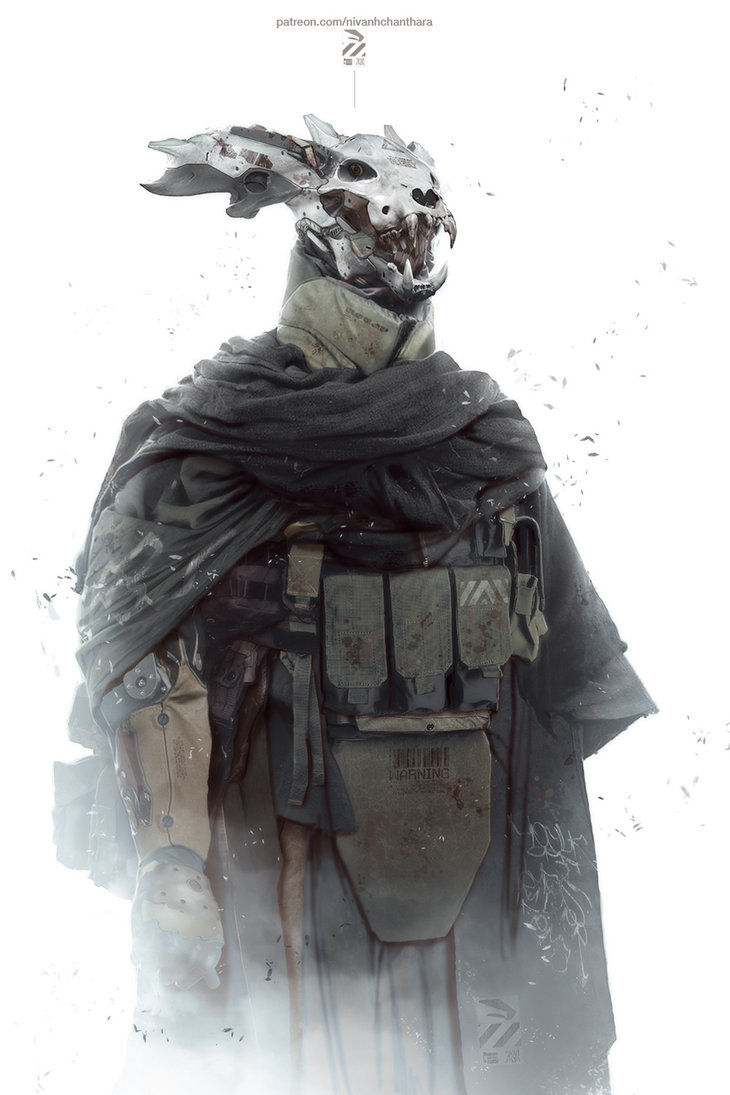
\includegraphics[width=0.5\textwidth]{figures/demo.jpg}
	\caption{demo的图片}\label{book}
	\vspace{-1em}
\end{figure}	

用以公式
\begin{align}
	f(a,b,c)=abc(100a+10b+c)\label{func}
\end{align}

其中\(a,b,c\in \mathbb{N}^+\)且\(a>b>c\),求函数~\eqref{func}~的值域。

\chapter{实验结果与讨论}
结论相关章节

\section{实验一}

\section{实验二}


\chapter{对更广泛应用的评估}
\section{总结}
\section{后续工作展望}


随着社会发展,有更多的⼯件材料被⽣产出来,对于表⾯的质量要求也逐渐 增⾼,表⾯的质量问题也逐渐被⼈们所关注,但是在⼯件⽣产过程中,收到⽣产 ⼯艺或者机器影响,⼯件上经常会出现凹陷、凸起、划痕等表⾯缺陷问题。因此 逐步形成了表⾯缺陷检测技术。表⾯缺陷检测技术是⾃动化⼯业⽣产中的重要 ⼀环,在整个⽣产环节中,产⽣表⾯缺陷,形成部件缺失或者是部件错位,除了 检测精度以外,在资源有限的⾃动表⾯检测解决⽅案上也需要在易⽤性和处理 时间⽅⾯也同时具有优异的性能。本⽂提出了⼀种基于 CornerNet 的神经⽹络结 构,⽤于检测⼀些常⻅的表⾯缺陷。在数据集的基础上,基于图像的降噪、预处 理和数据增强,增加数据的可⽤性。并使⽤多层的 fire module ⽤以优化⽹络,并 使⽤ Hourglass 模块构建整个⽹络结构,通过深层可分离卷积⽤以降低整个⽹络 的运算需求,也提⾼了整个模型的检测精度。实验表明,与主流的卷积神经⽹络
相⽐,我们的模型精确性和实时性都有保证,能够满⾜表⾯缺陷检测的要求。

With the development of morden society, more workpiece are produced, and the surface quality requirements are increasing. To stand test of time, the quality of surface is gradually concerned by people. However, After production process, workpiece may take damage due to the production process and influence of machine,Such as depressions, bumps, and scratches often occur on the workpiece. Therefore, surface defect detection technology has gradually formed and become an important part of automated industrial production. In the production process, missing parts or parts are dislocated may be the surface defects. Despite detection accuracy, it is also required in automatic surface inspection solutions with limited resources. It also need to have excellent performance in terms of ease of use as well as that in processing time. This paper presents a neural network structure based on CornerNet for detecting some common surface defects. Based on the dagm dataset, noise reduction, pre-processing and image augmentation are applyed to incerase data credibility. The entire network structure is built with the hourglass module, and multi-layer fire modules are included to optimize our network. The deep separable convolution reduces the computational requirements of the entire network and improves the detection accuracy of the entire model. Compared with the mainstream convolutional neural network, our model is seemed to be more accurate and better in real-time test, which meet the requirements of surface defect
detection.

表⾯缺陷;机器视觉;深度学习;图像处理;神经⽹络; surface defect; machine Vision; deep learning; Image Processing; nerual network




%%%%%%%%%%  参考文献  %%%%%%%%%%
\makereferences

%%%%%%%%%%    附录    %%%%%%%%%%
\titleformat{\chapter}{\centering\sihao\hei}{\chaptername}{2em}{} % 标题四号黑体居中
% !Mode:: "TeX:UTF-8"

\titlecontents{chapter}[2em]{\vspace{.5\baselineskip}\xiaosan\song}%
             {\prechaptername\CJKnumber{\thecontentslabel}\postchaptername\qquad}{} %
             {}             % 设置该选项为空是为了不让目录中显示页码          
\addcontentsline{toc}{chapter}{外文资料}
%\setcounter{page}{1}       % 如果需要从该页开始从 1 开始编页,则取消该注释
\markboth{外文资料}{外文资料}
\chapter*{外文资料}

\includepdf[pages=-]{include/english.pdf}

% \begin{figure}[!b]
%     \centering
%     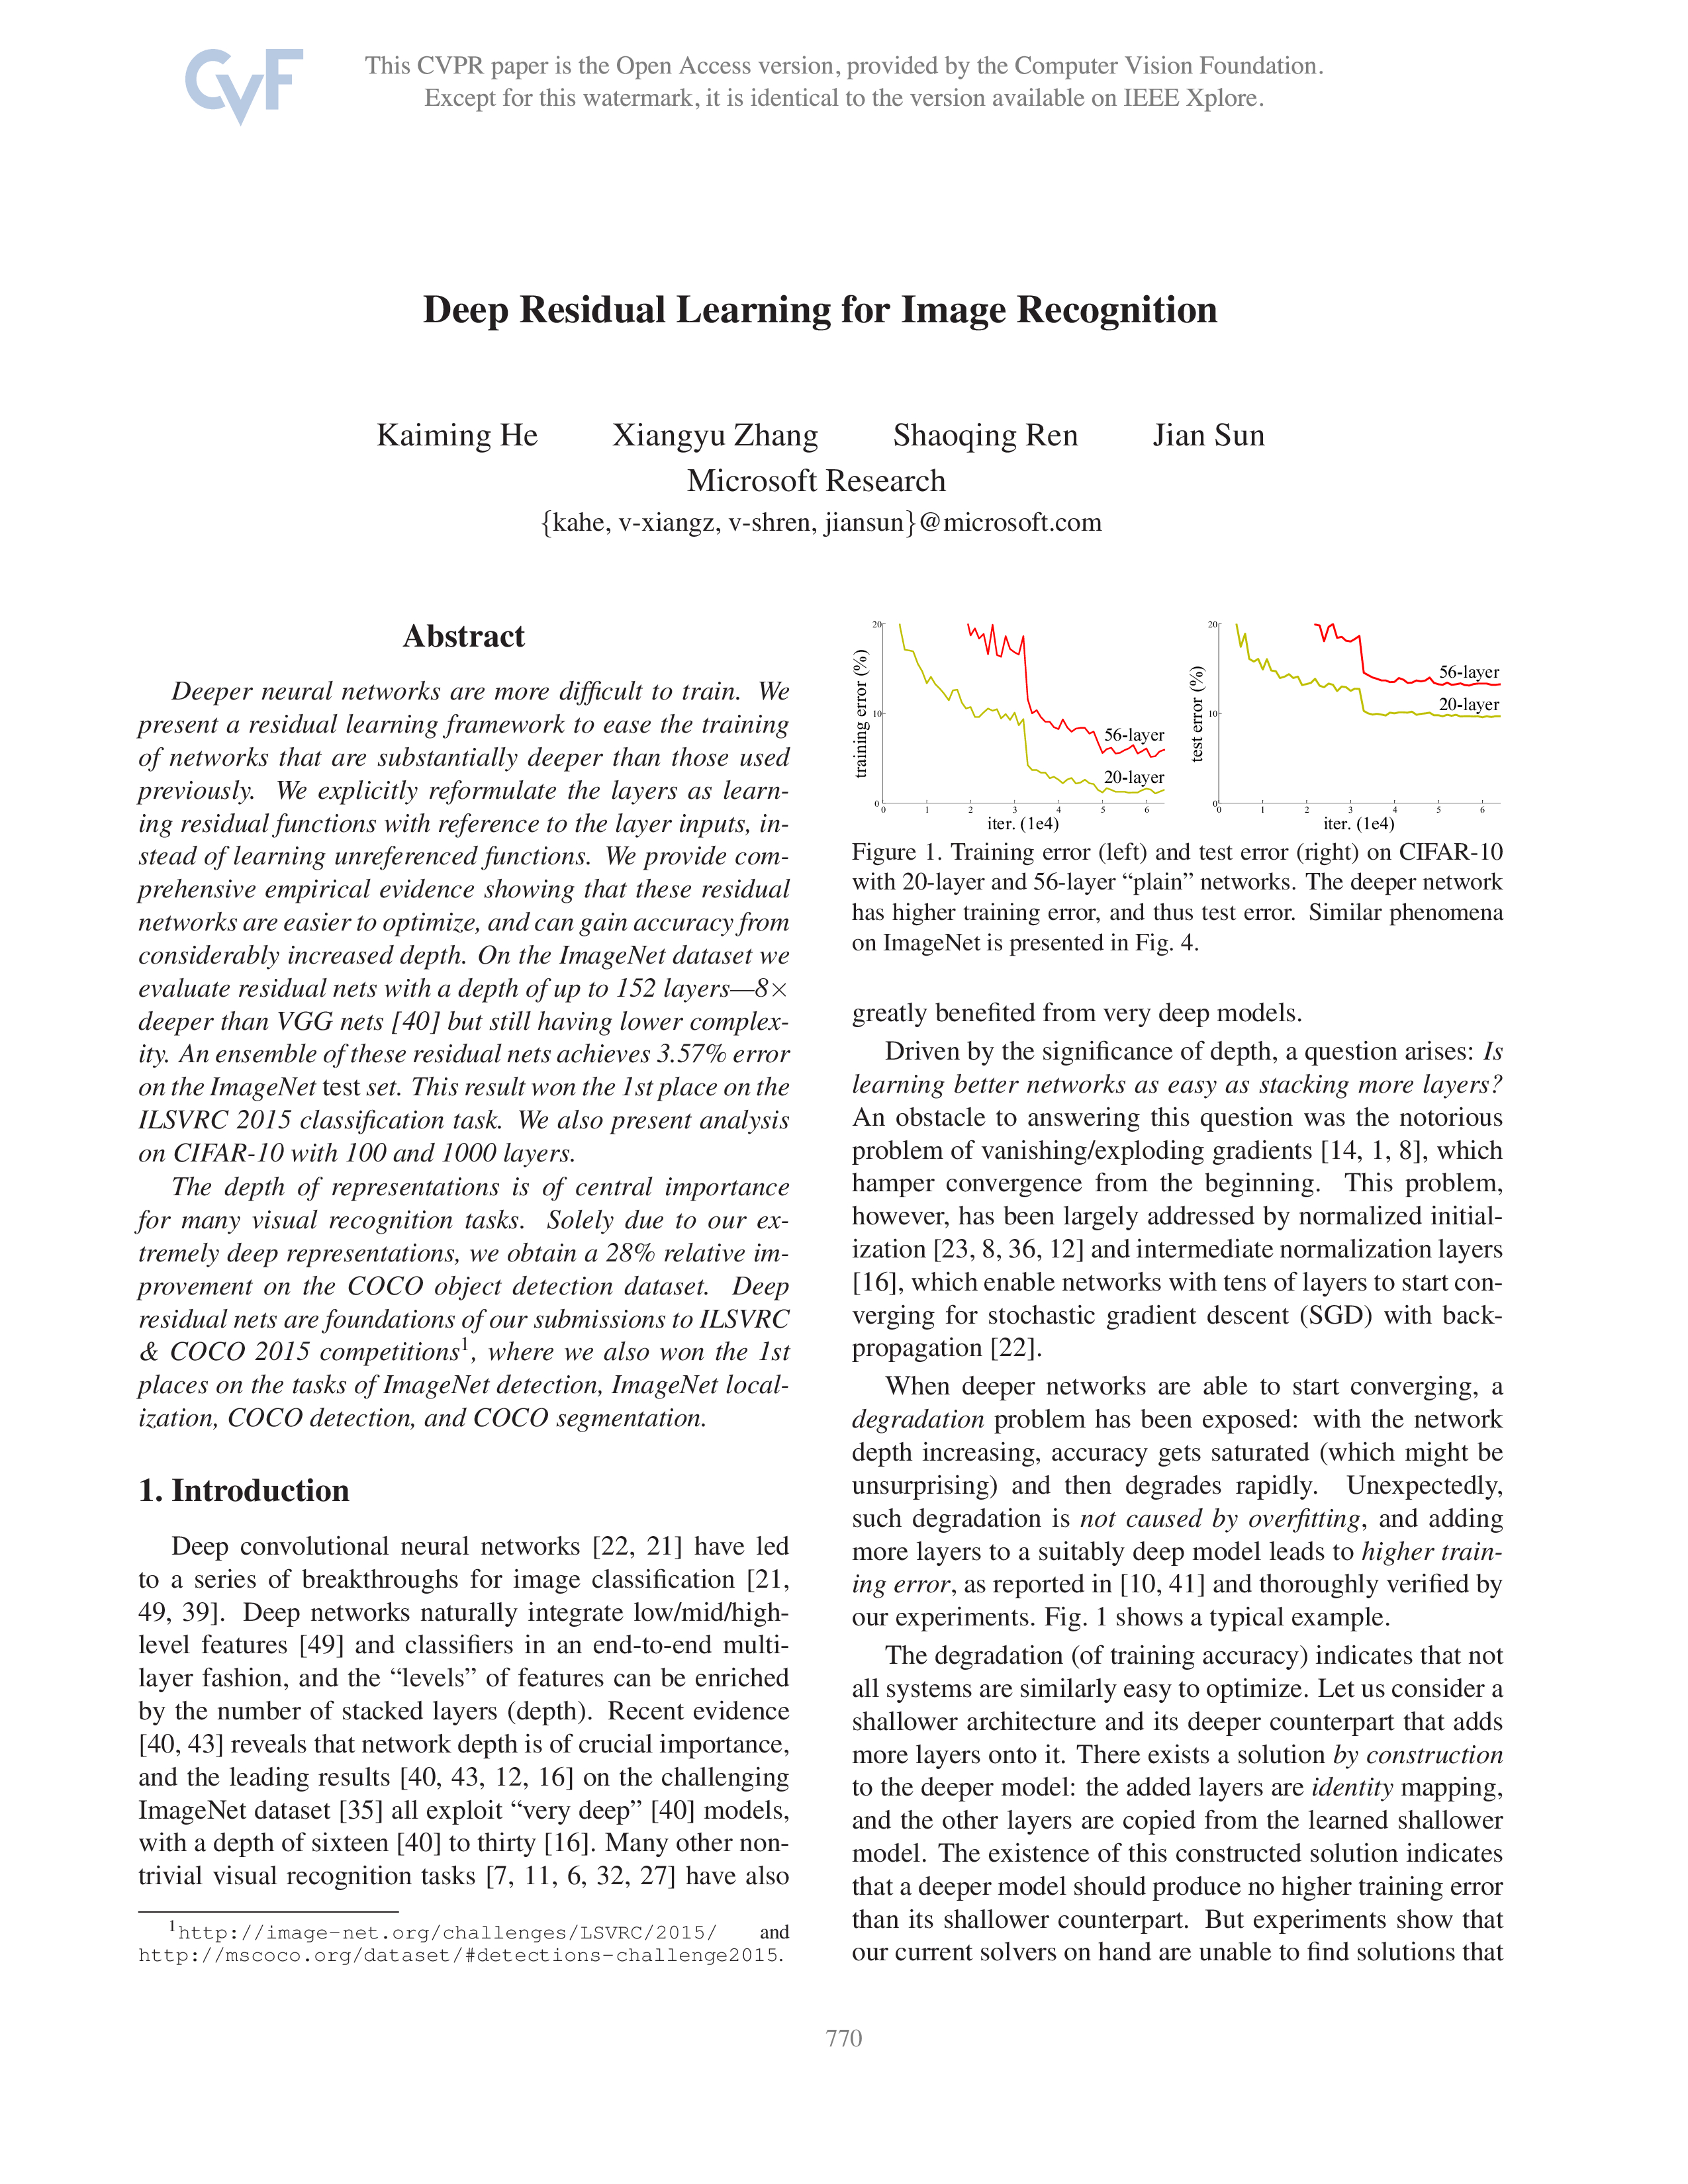
\includegraphics[width=\textwidth]{figures/english/english-0.jpg}
% \end{figure}

% \newpage

% \begin{figure}[!tbp]
%     \centering
%     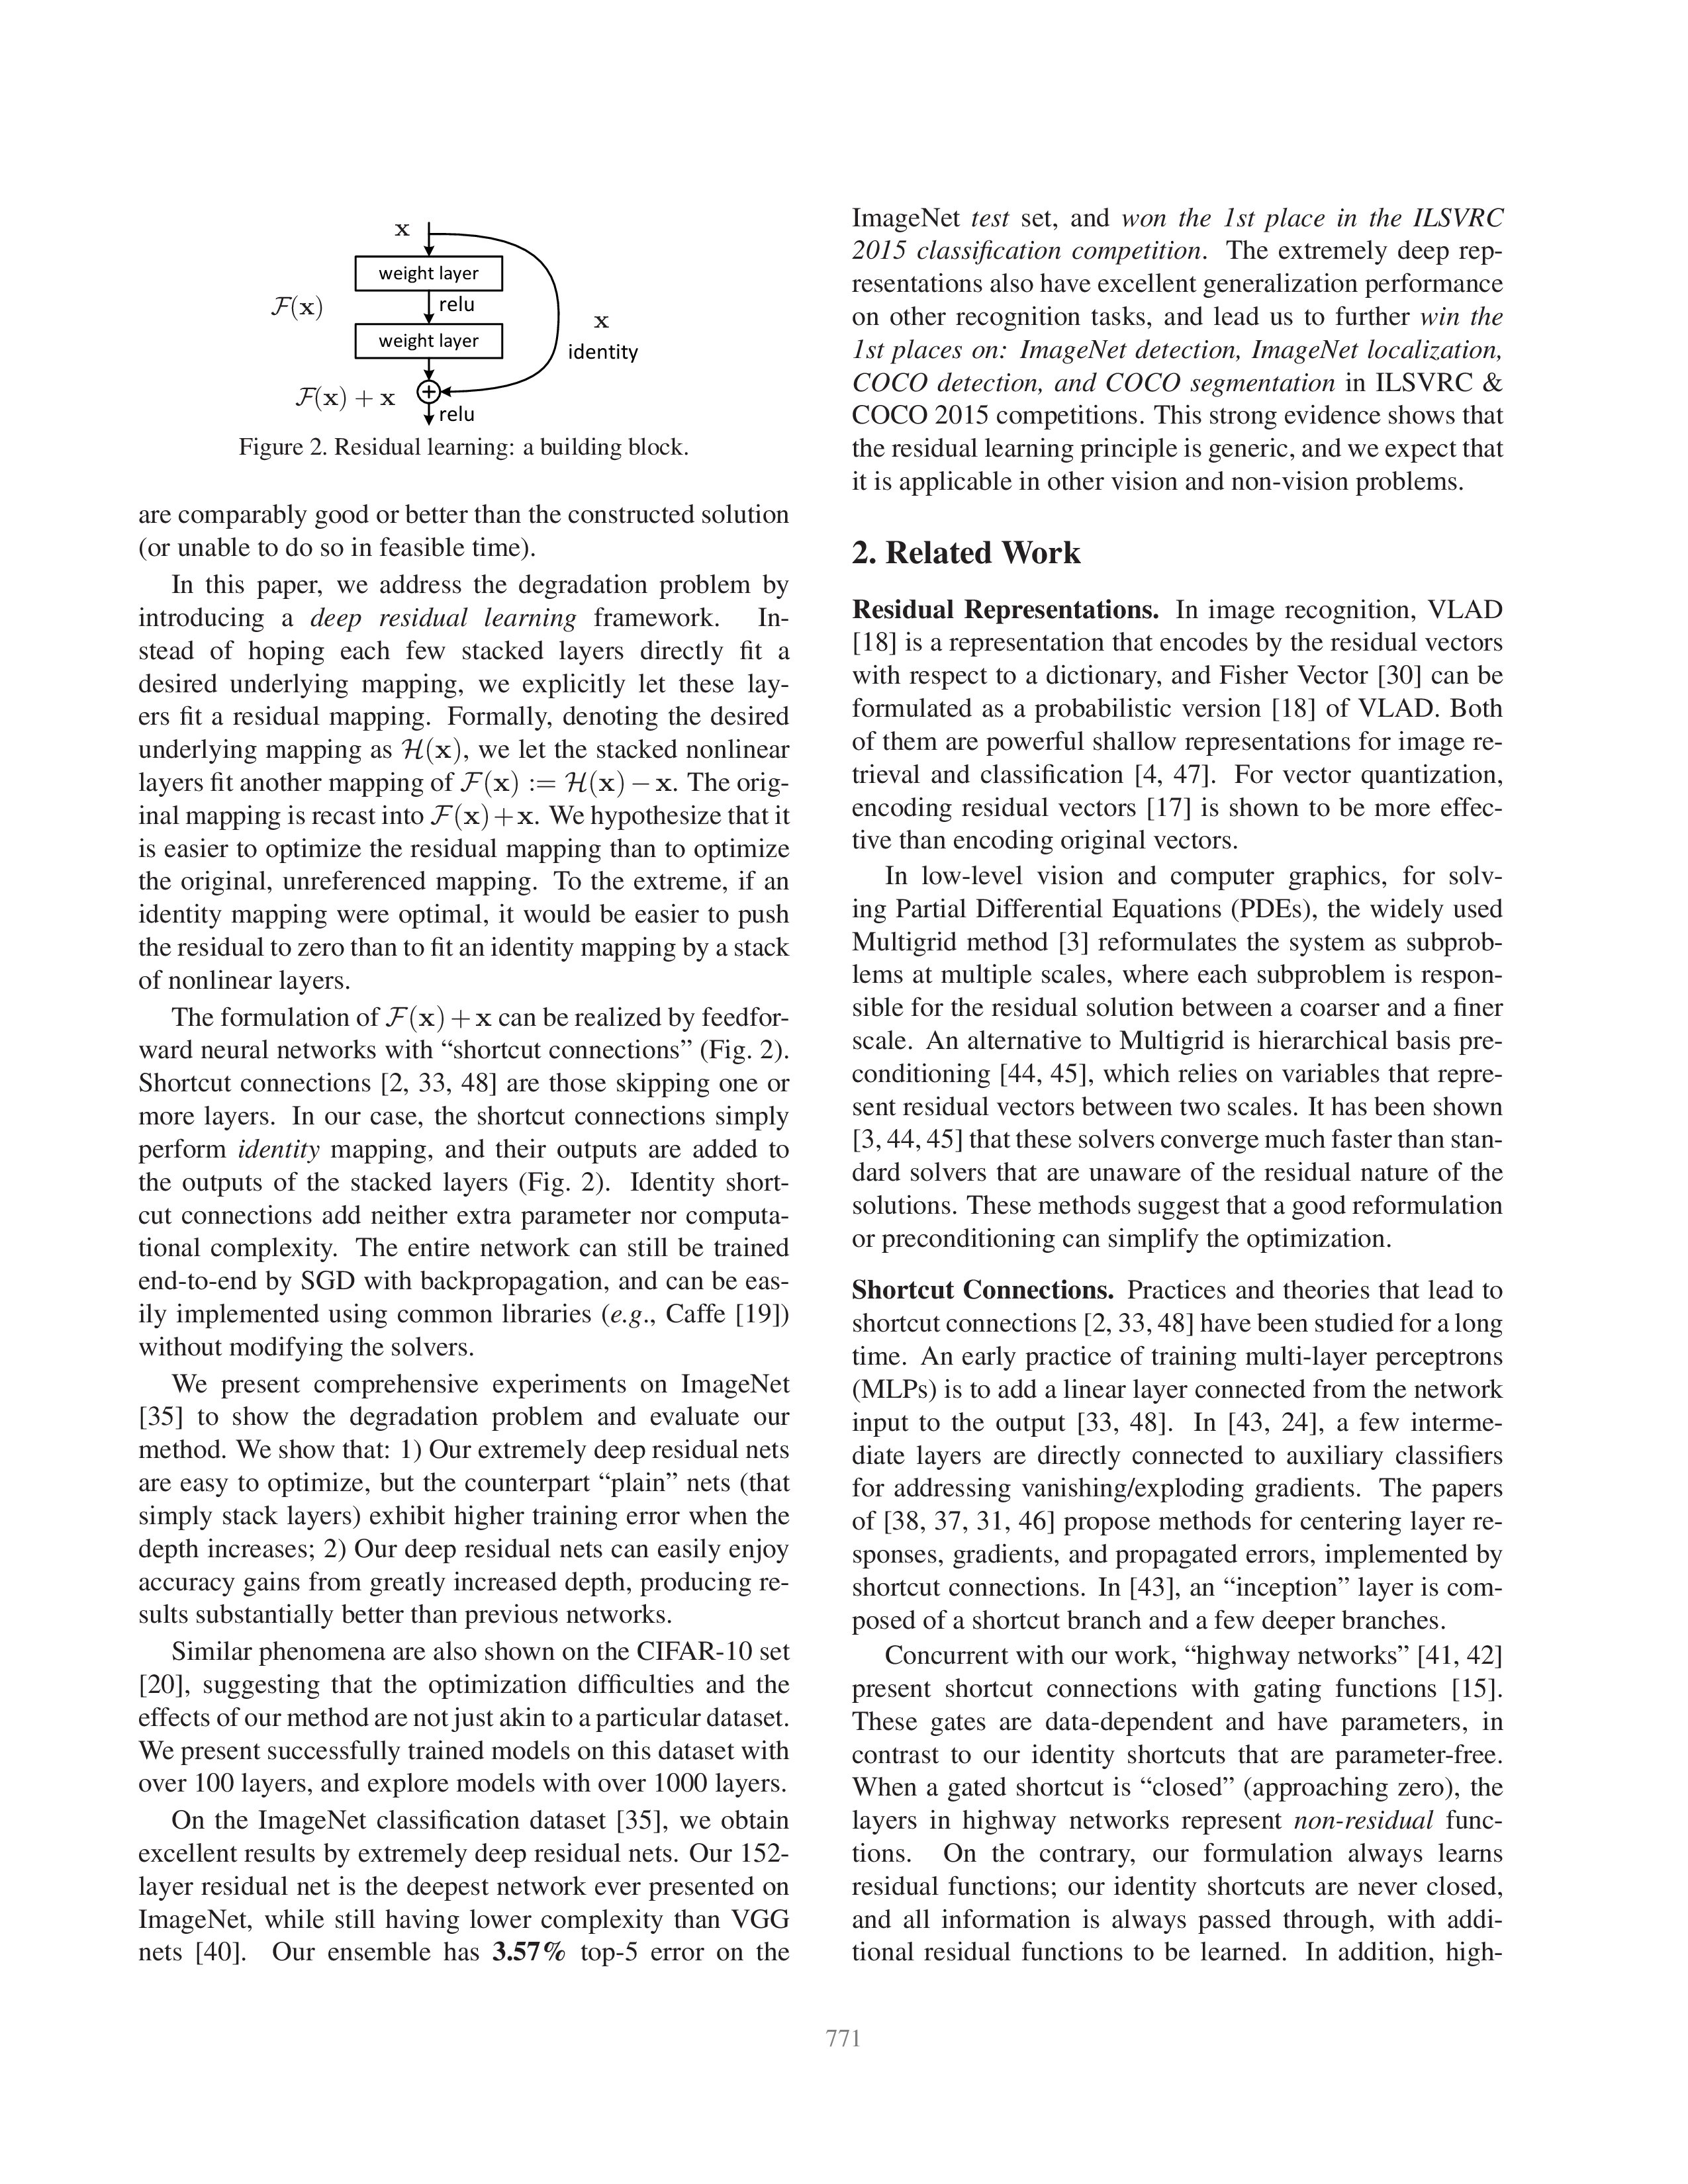
\includegraphics[width=\textwidth]{figures/english/english-1.jpg}
% \end{figure}

% \begin{figure}[!tbp]
%     \centering
%     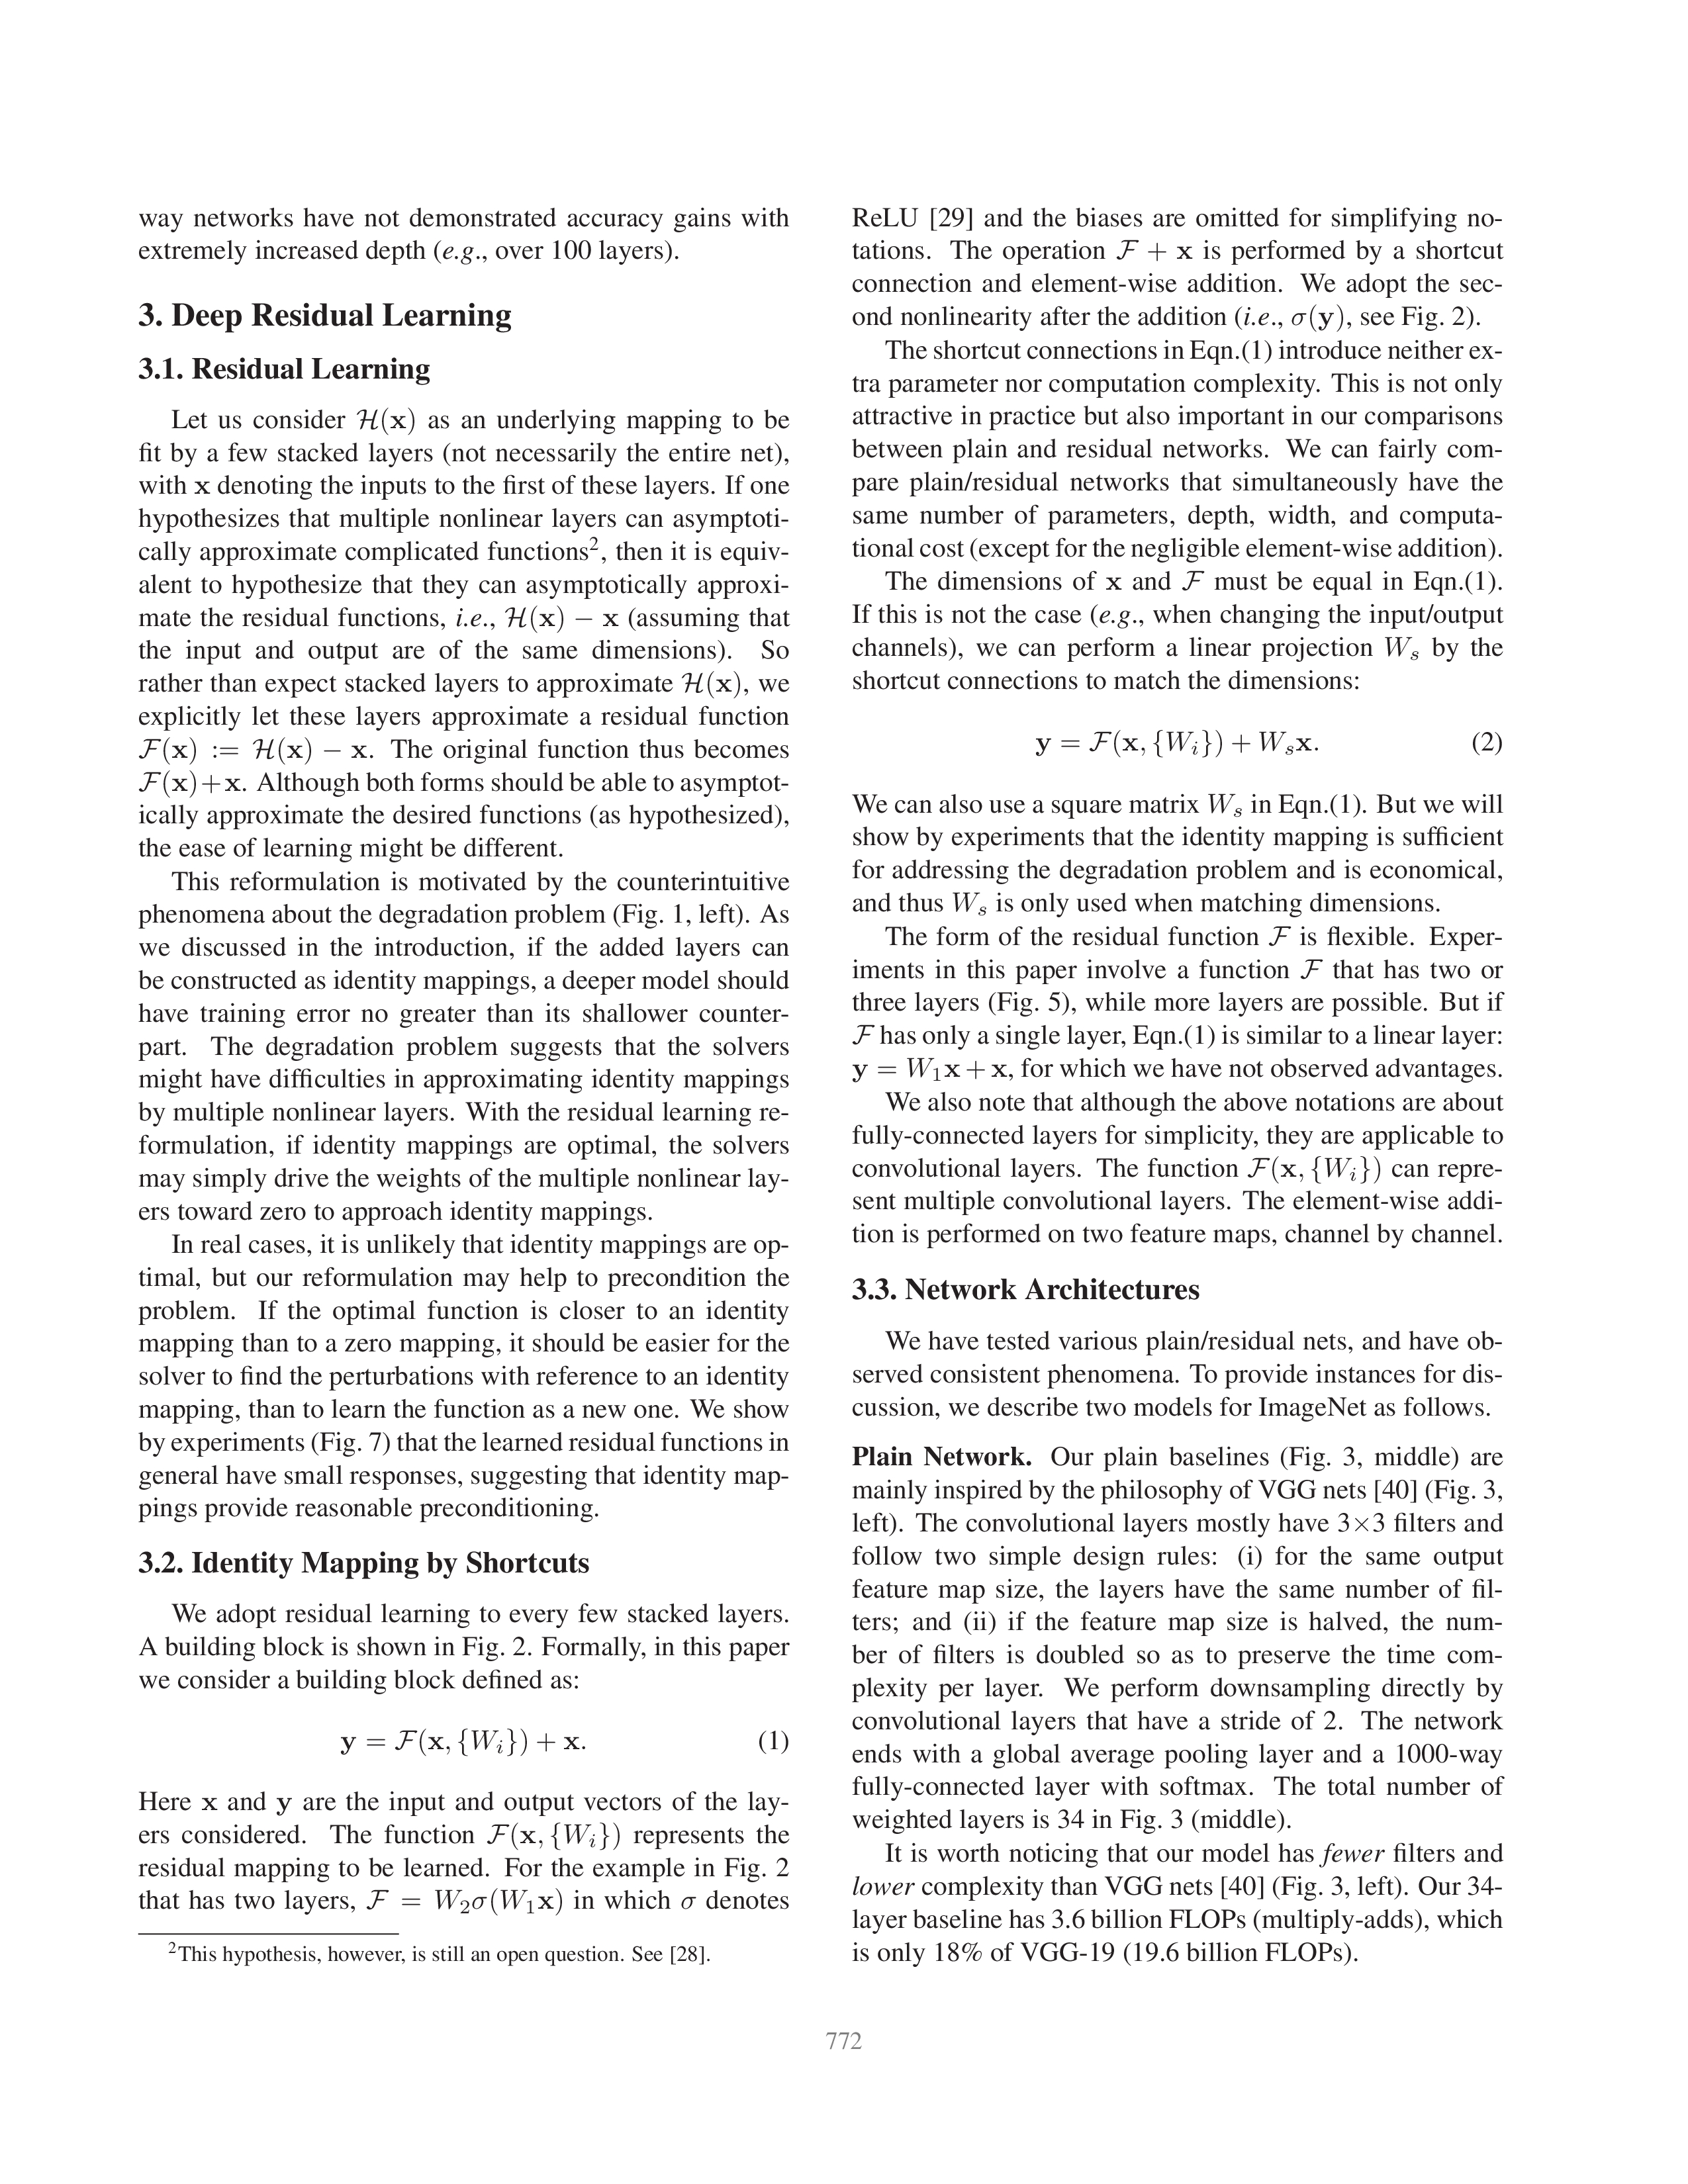
\includegraphics[width=\textwidth]{figures/english/english-2.jpg}
% \end{figure}

% \begin{figure}[!tbp]
%     \centering
%     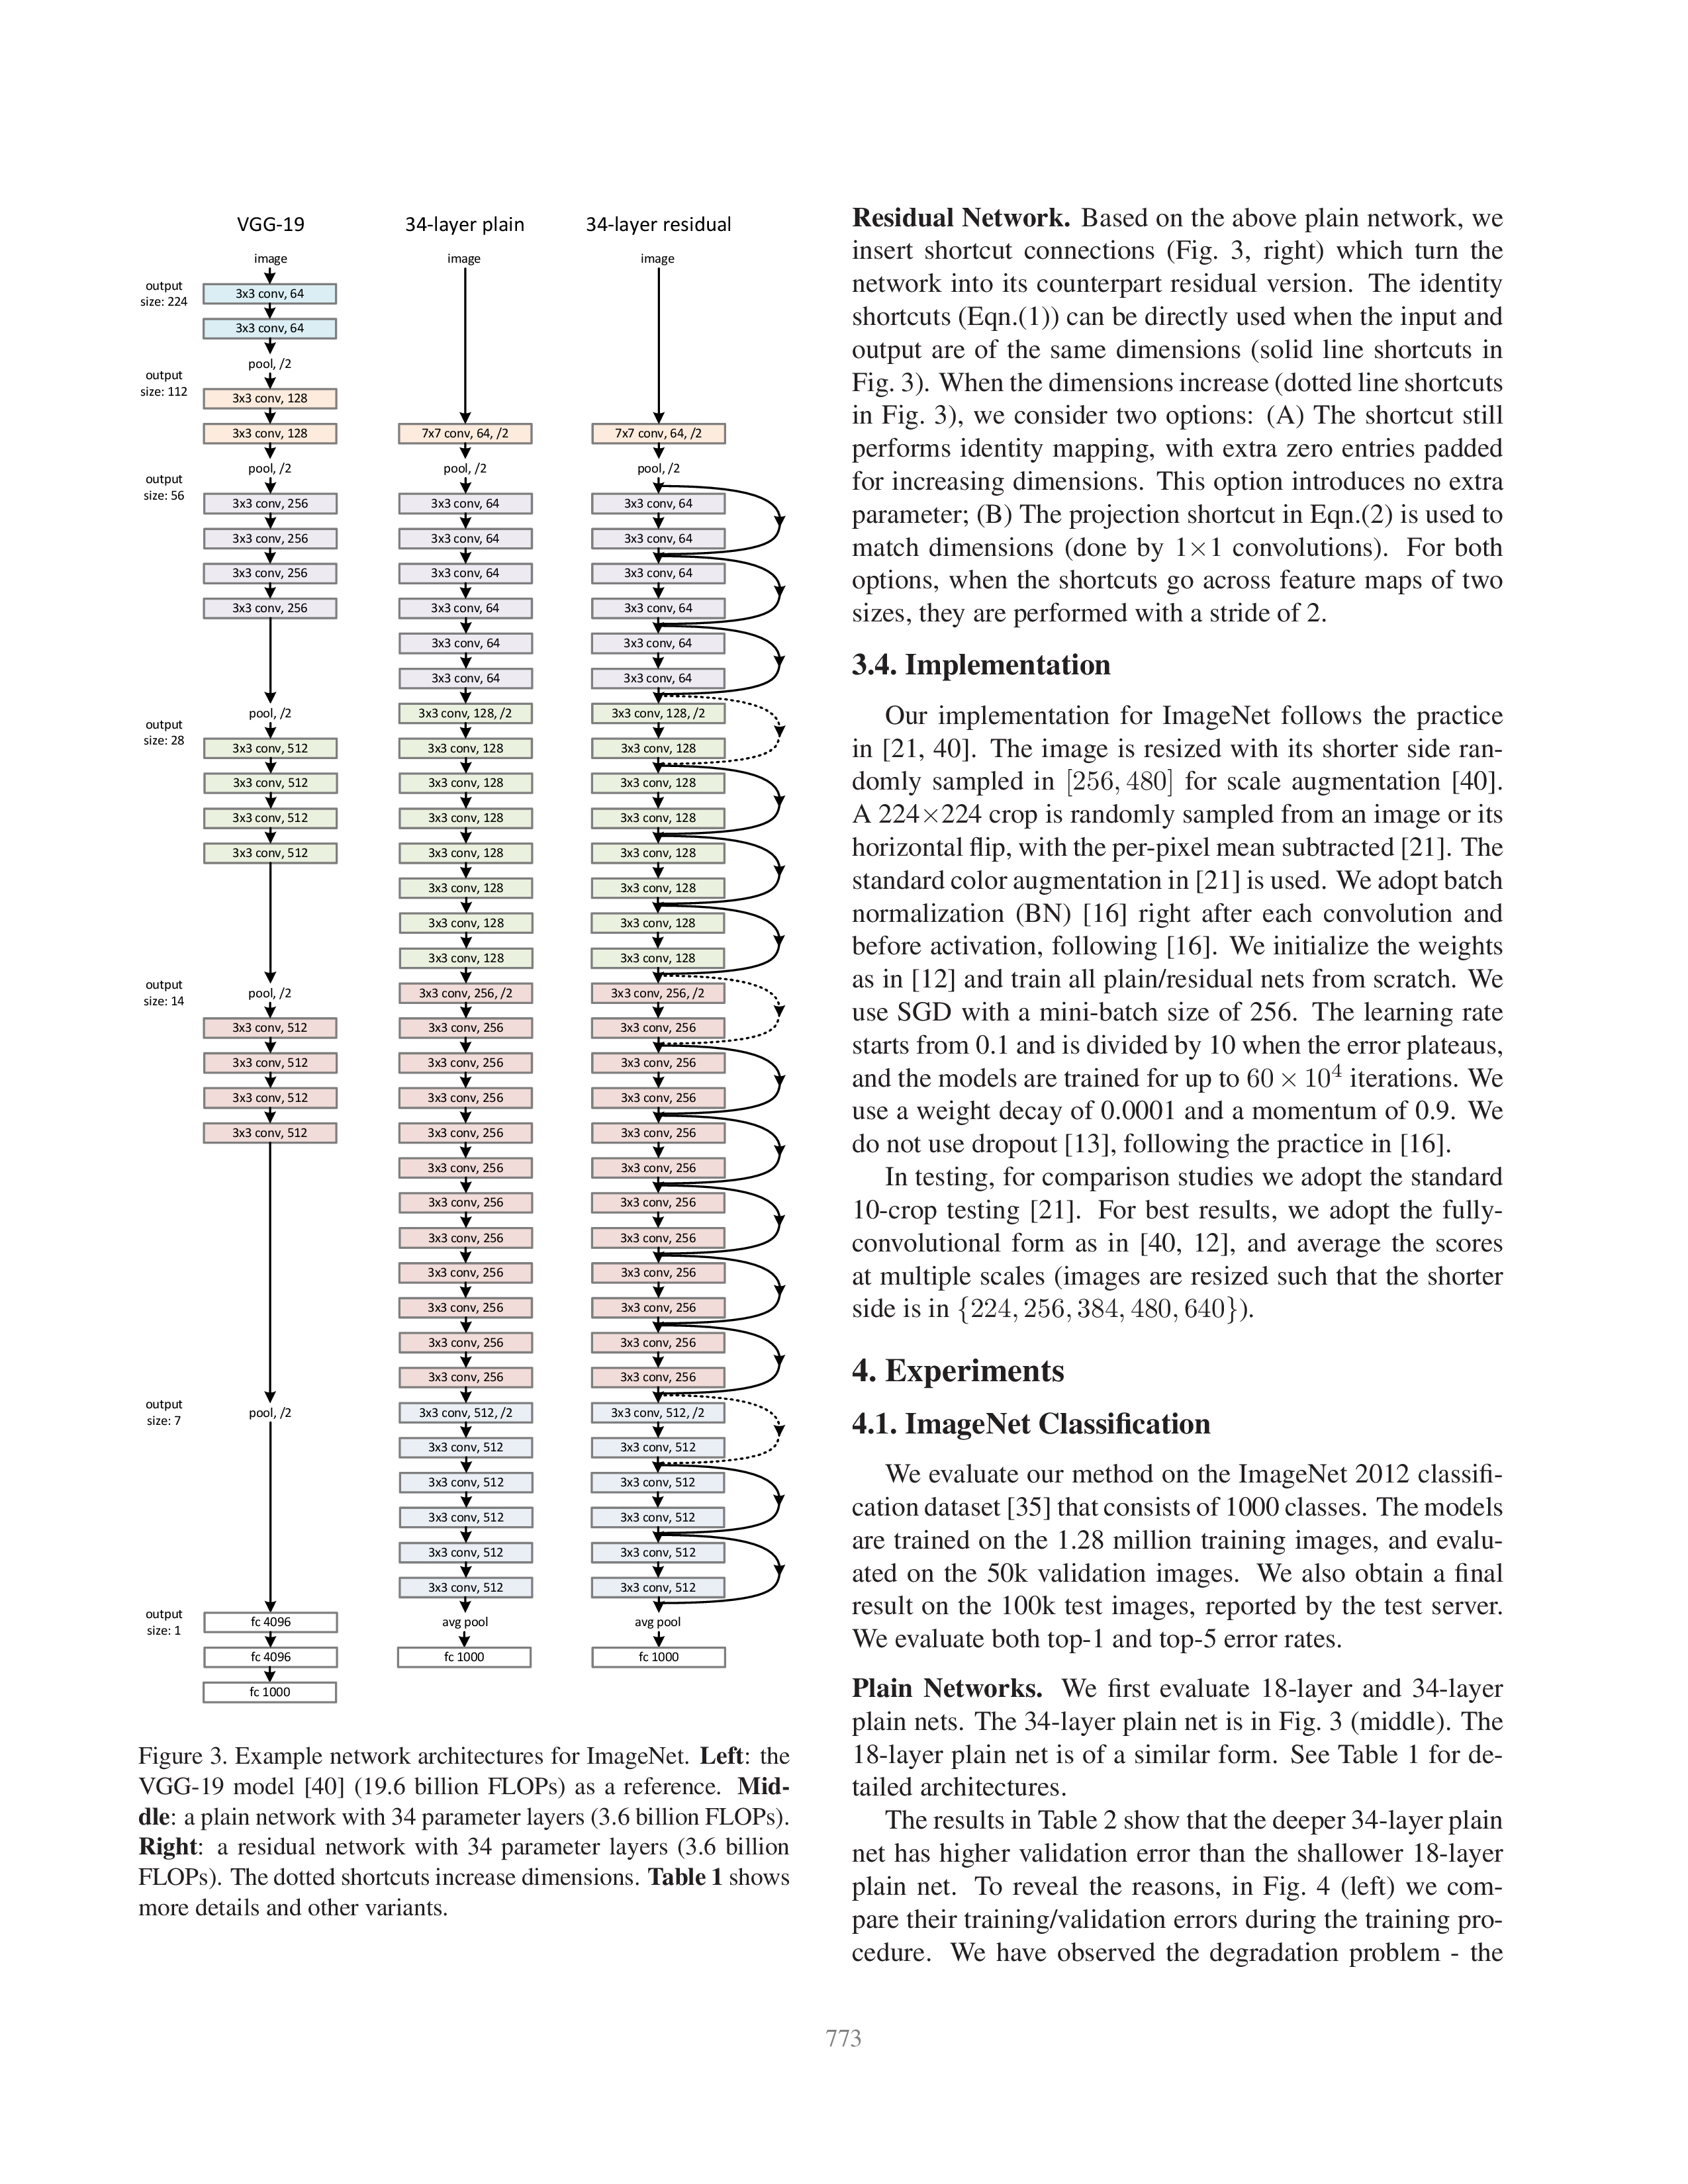
\includegraphics[width=\textwidth]{figures/english/english-3.jpg}
% \end{figure}

% \begin{figure}[!tbp]
%     \centering
%     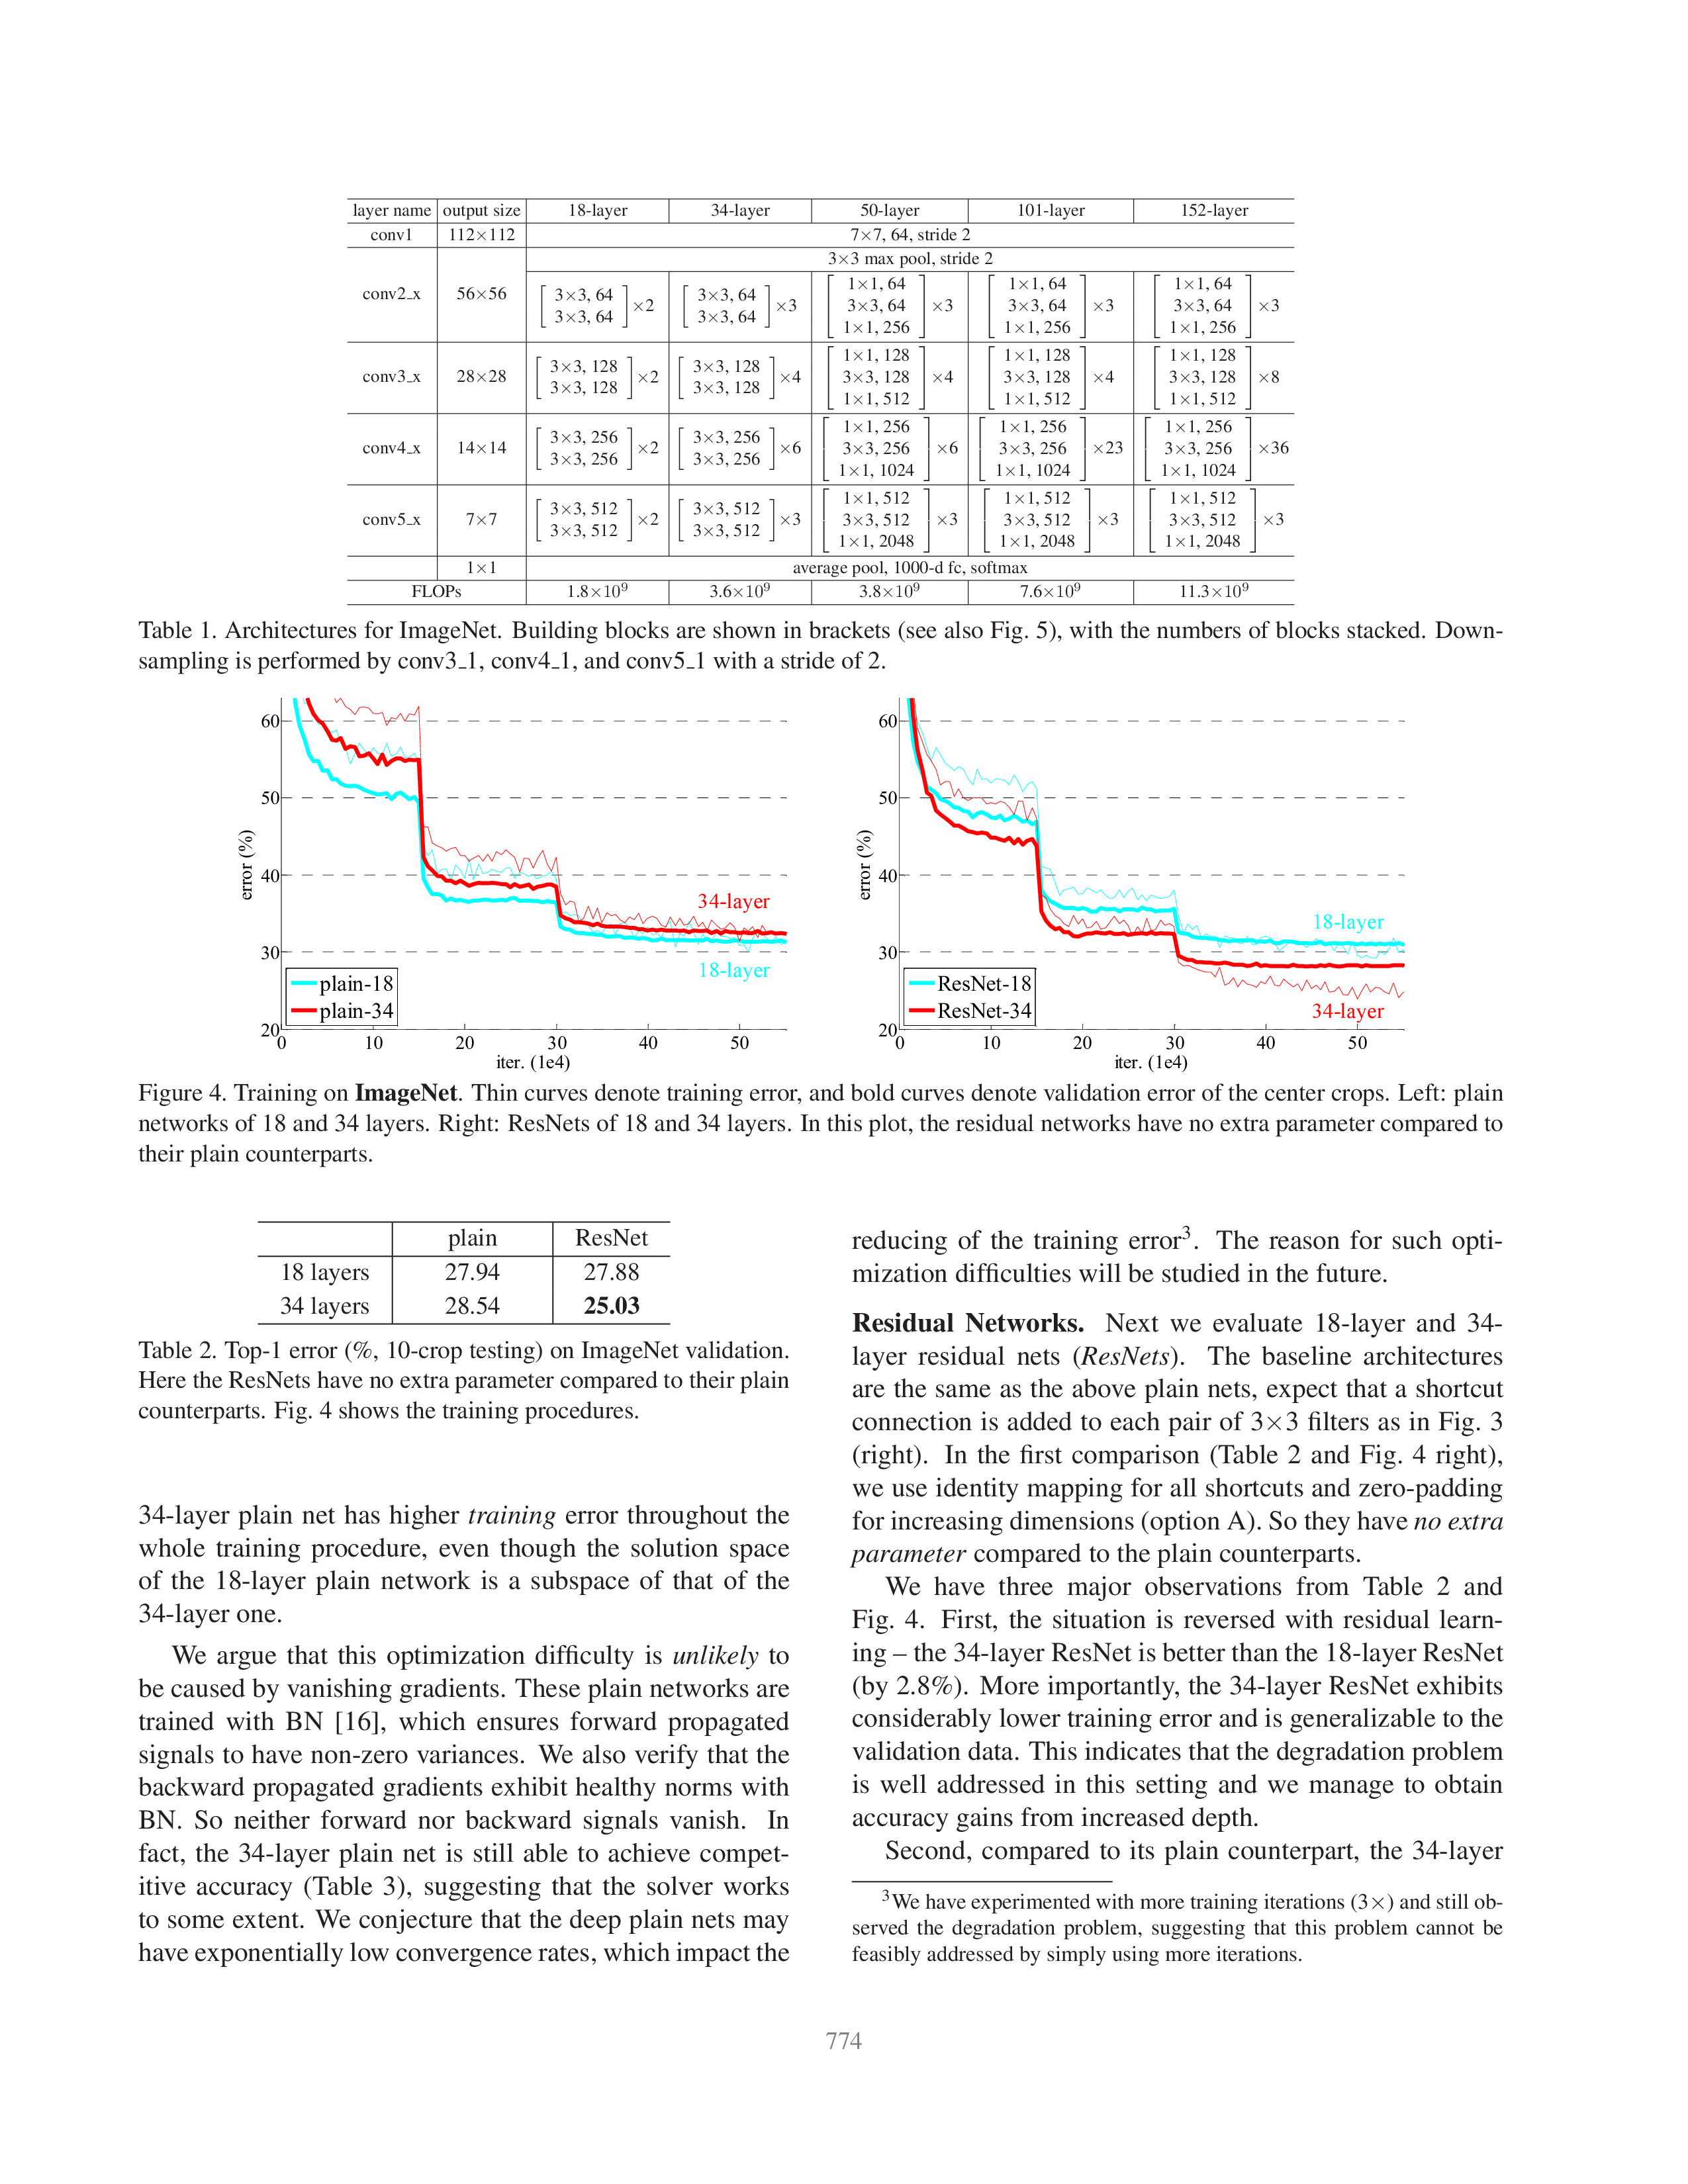
\includegraphics[width=\textwidth]{figures/english/english-4.jpg}
% \end{figure}

% \begin{figure}[!tbp]
%     \centering
%     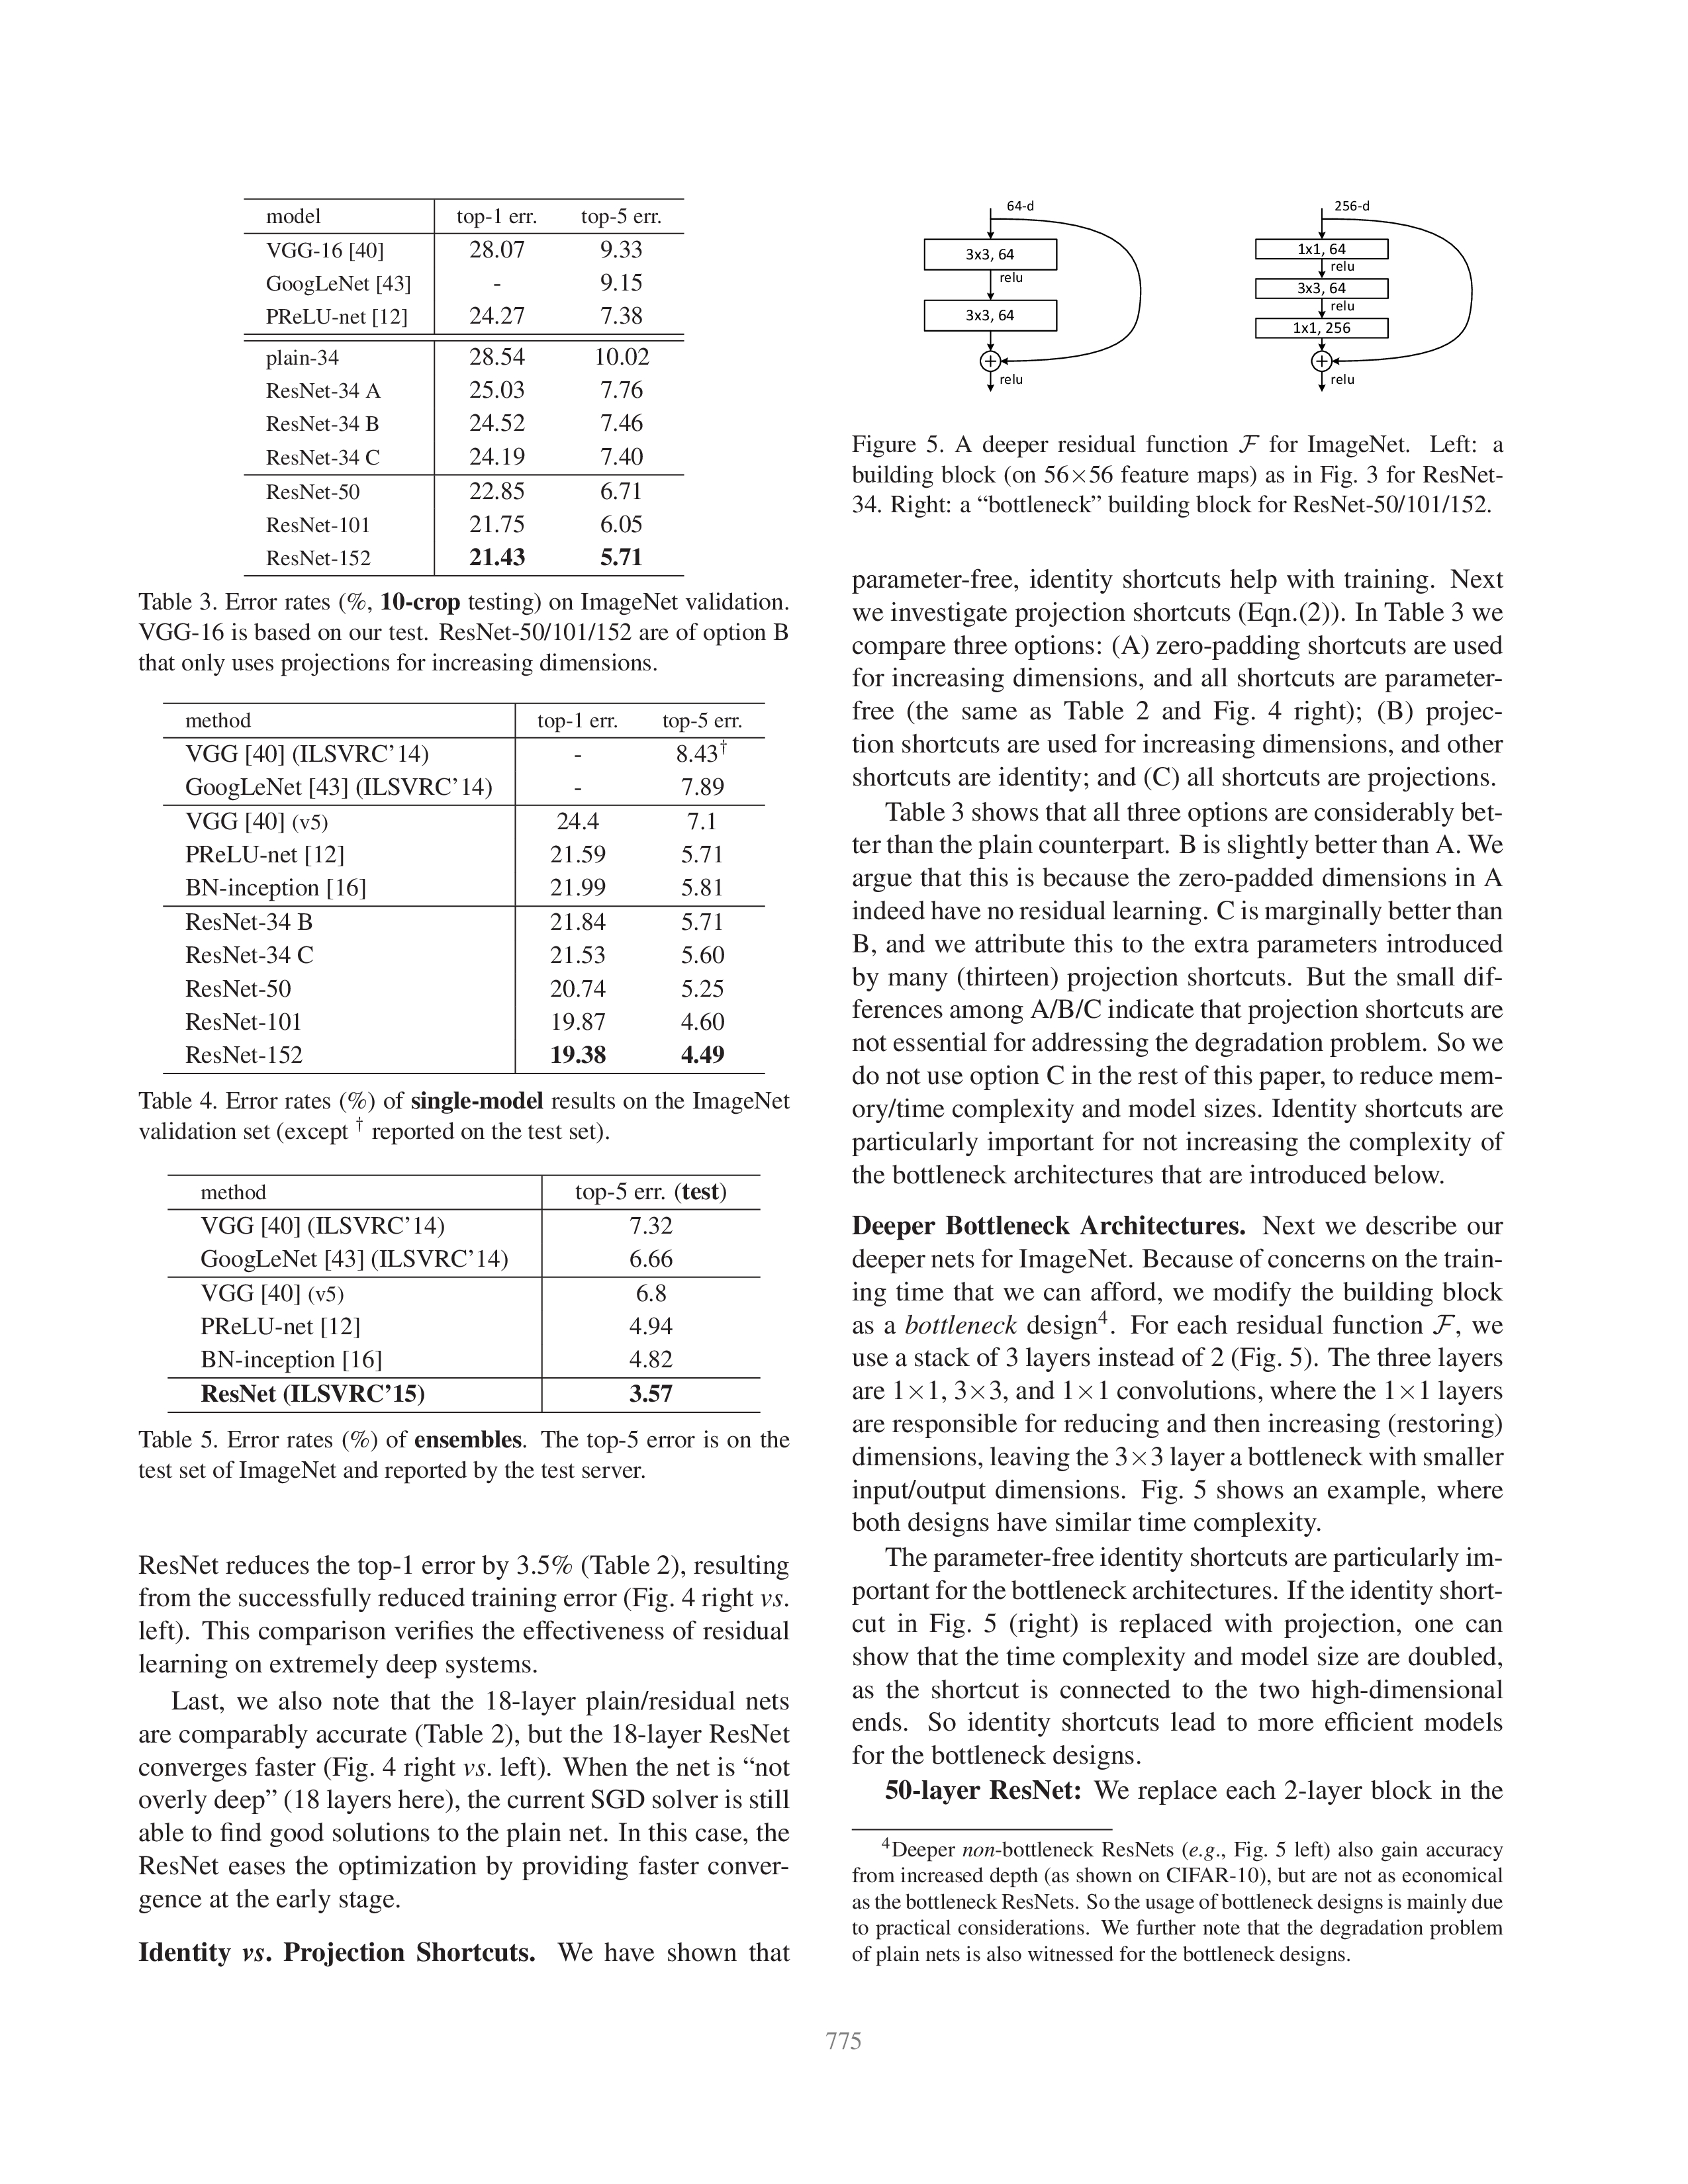
\includegraphics[width=\textwidth]{figures/english/english-5.jpg}
% \end{figure}

% \begin{figure}[!tbp]
%     \centering
%     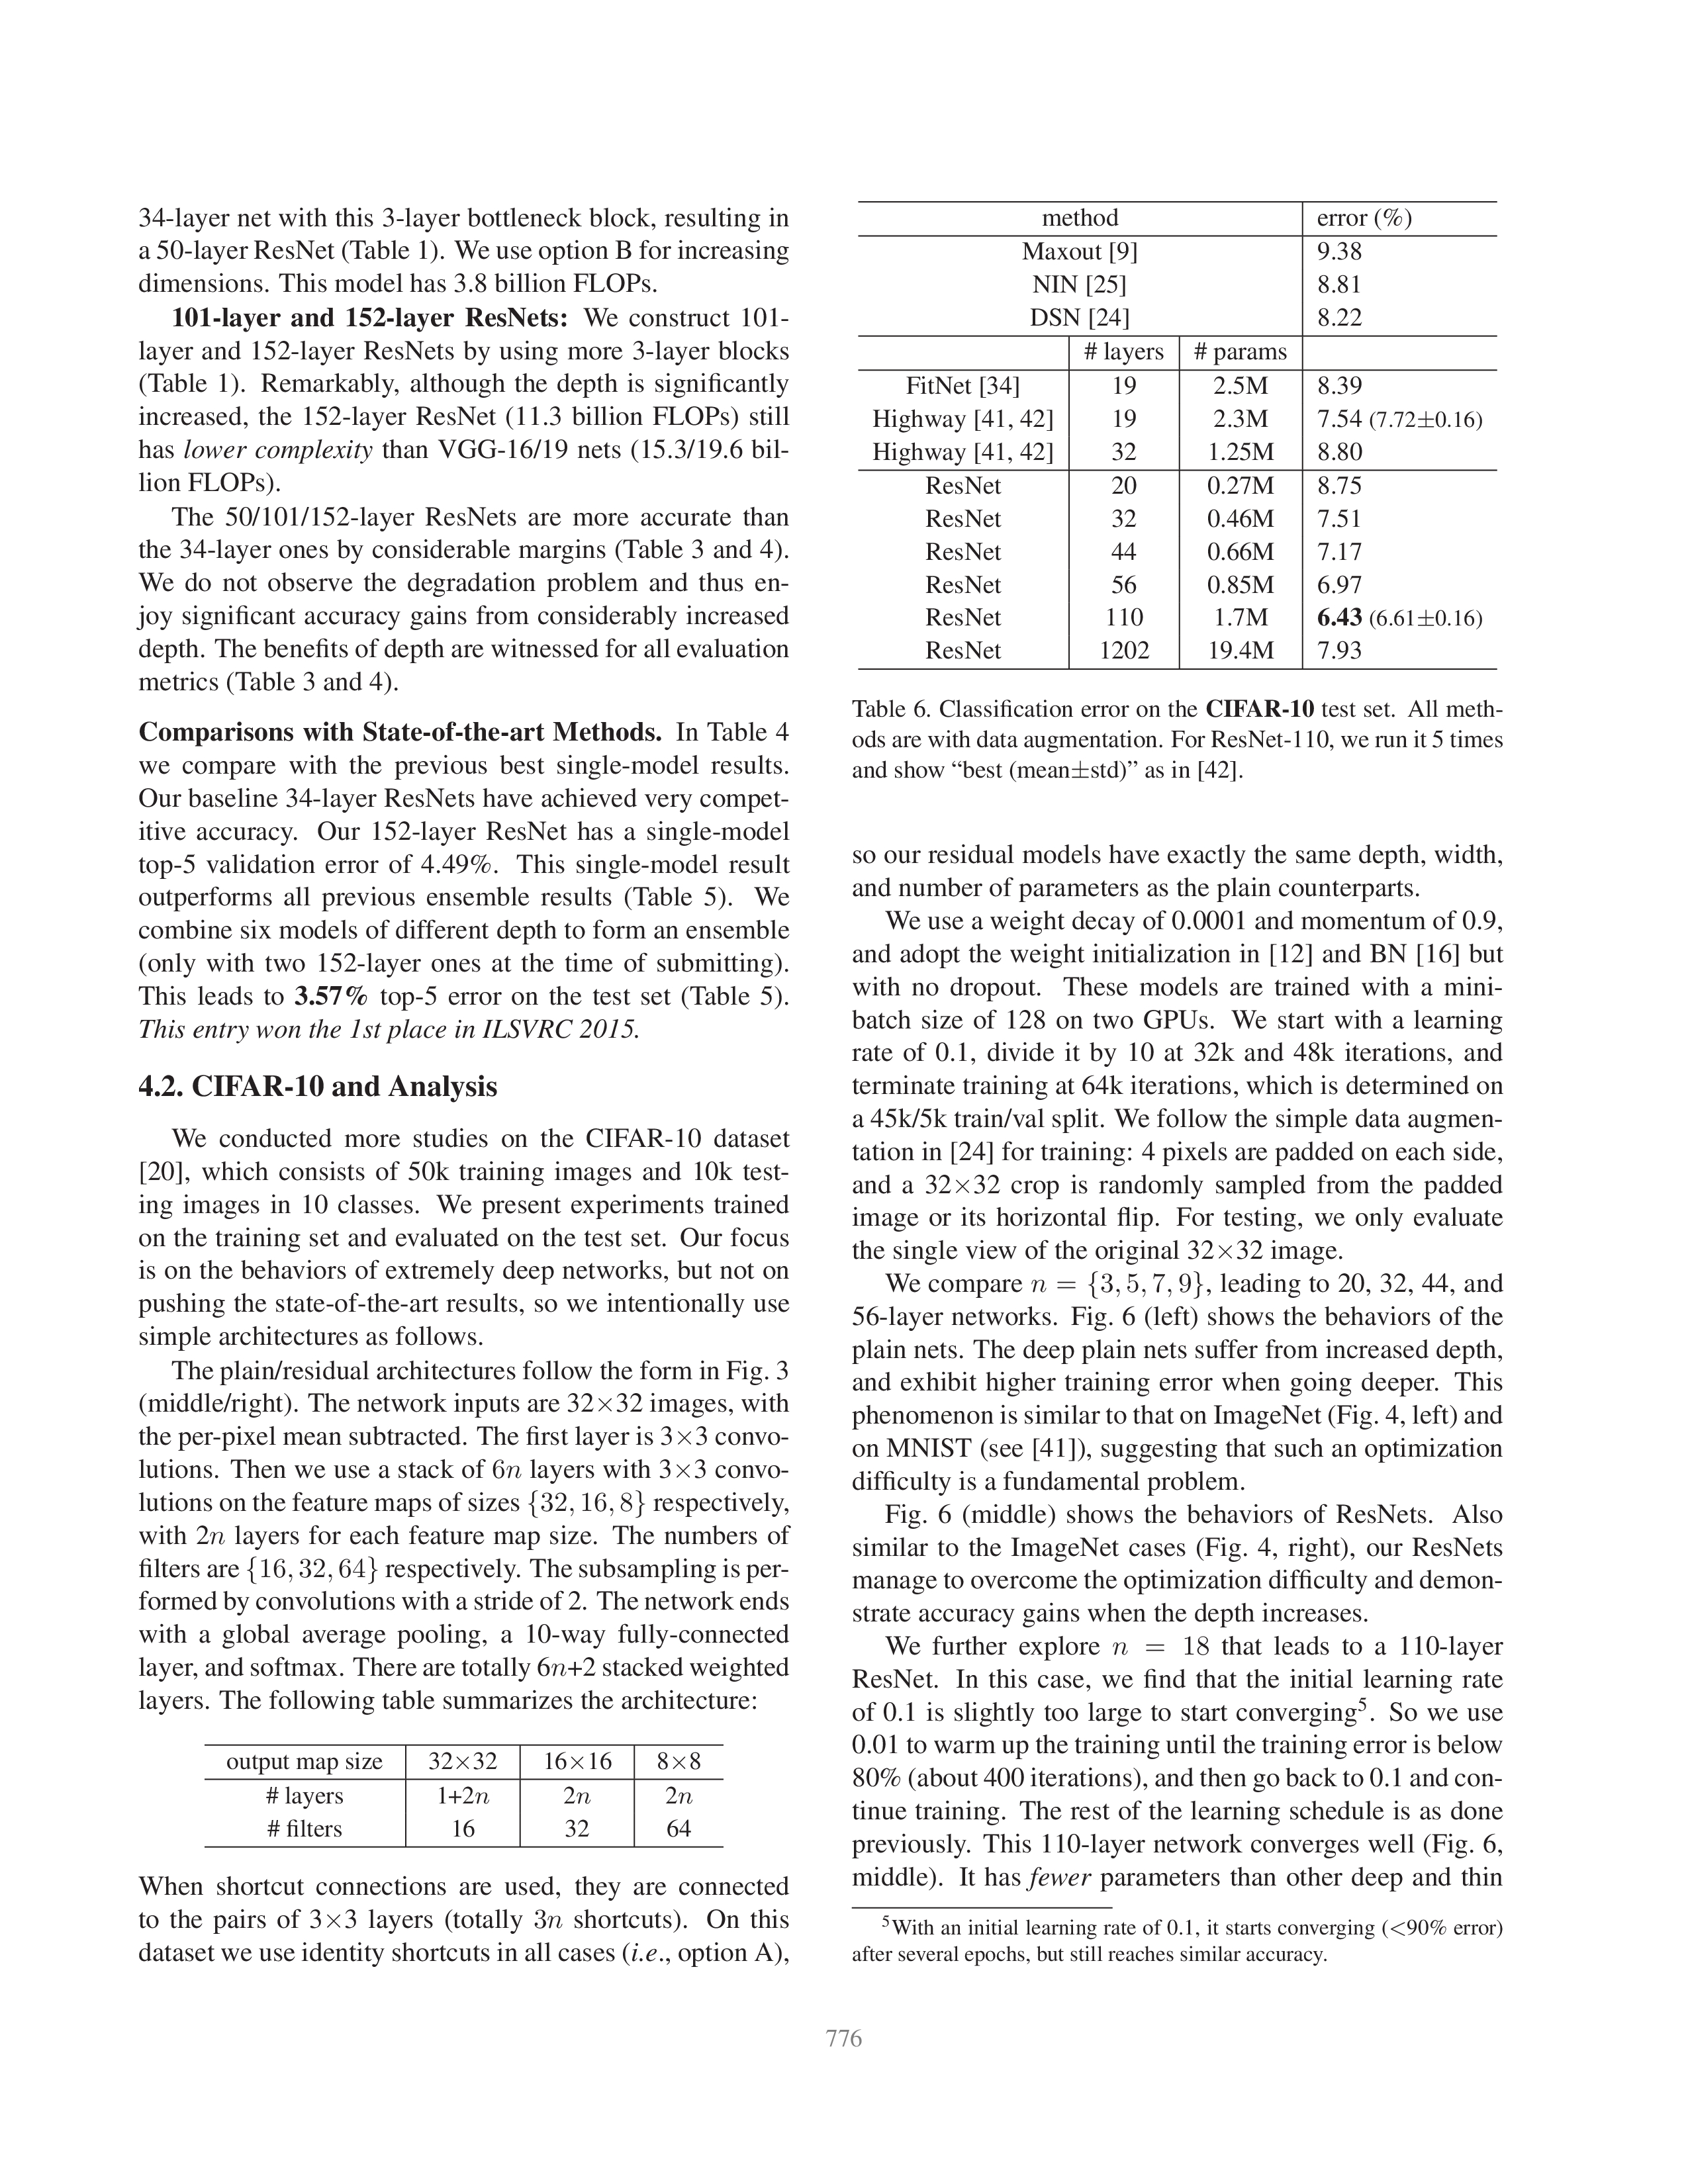
\includegraphics[width=\textwidth]{figures/english/english-6.jpg}
% \end{figure}

% \begin{figure}[!tbp]
%     \centering
%     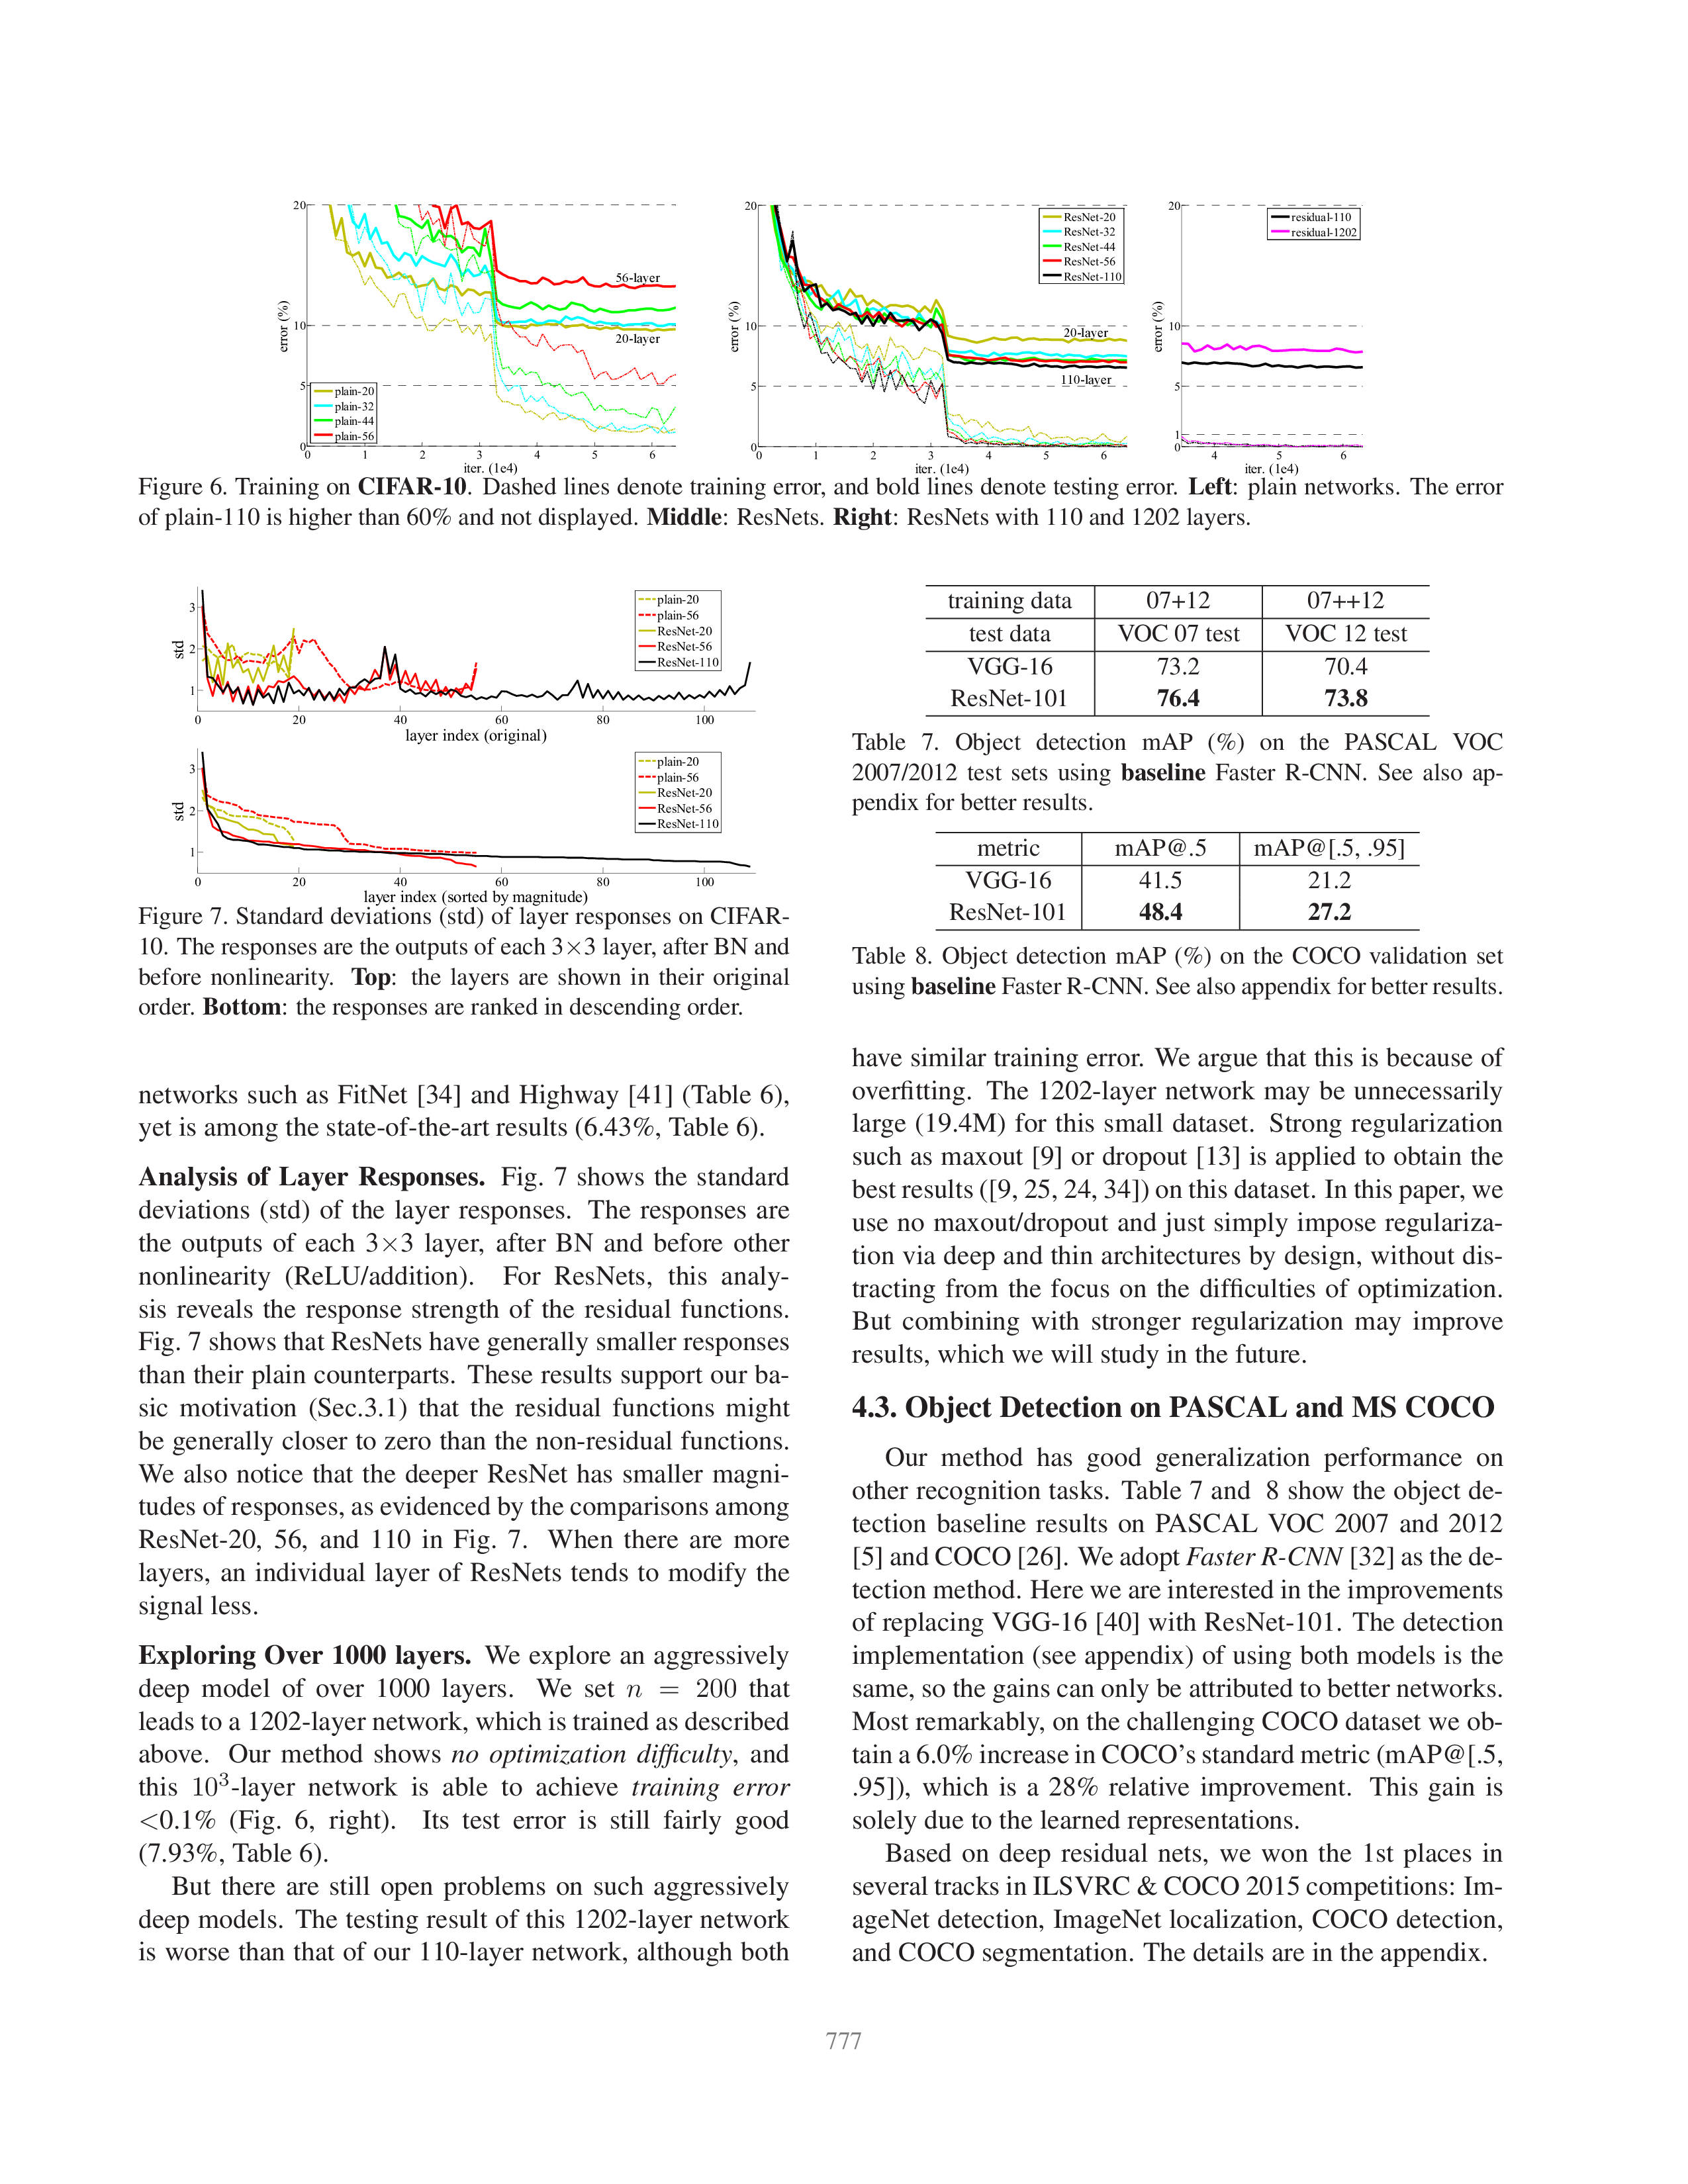
\includegraphics[width=\textwidth]{figures/english/english-7.jpg}
% \end{figure}

% \begin{figure}[!tbp]
%     \centering
%     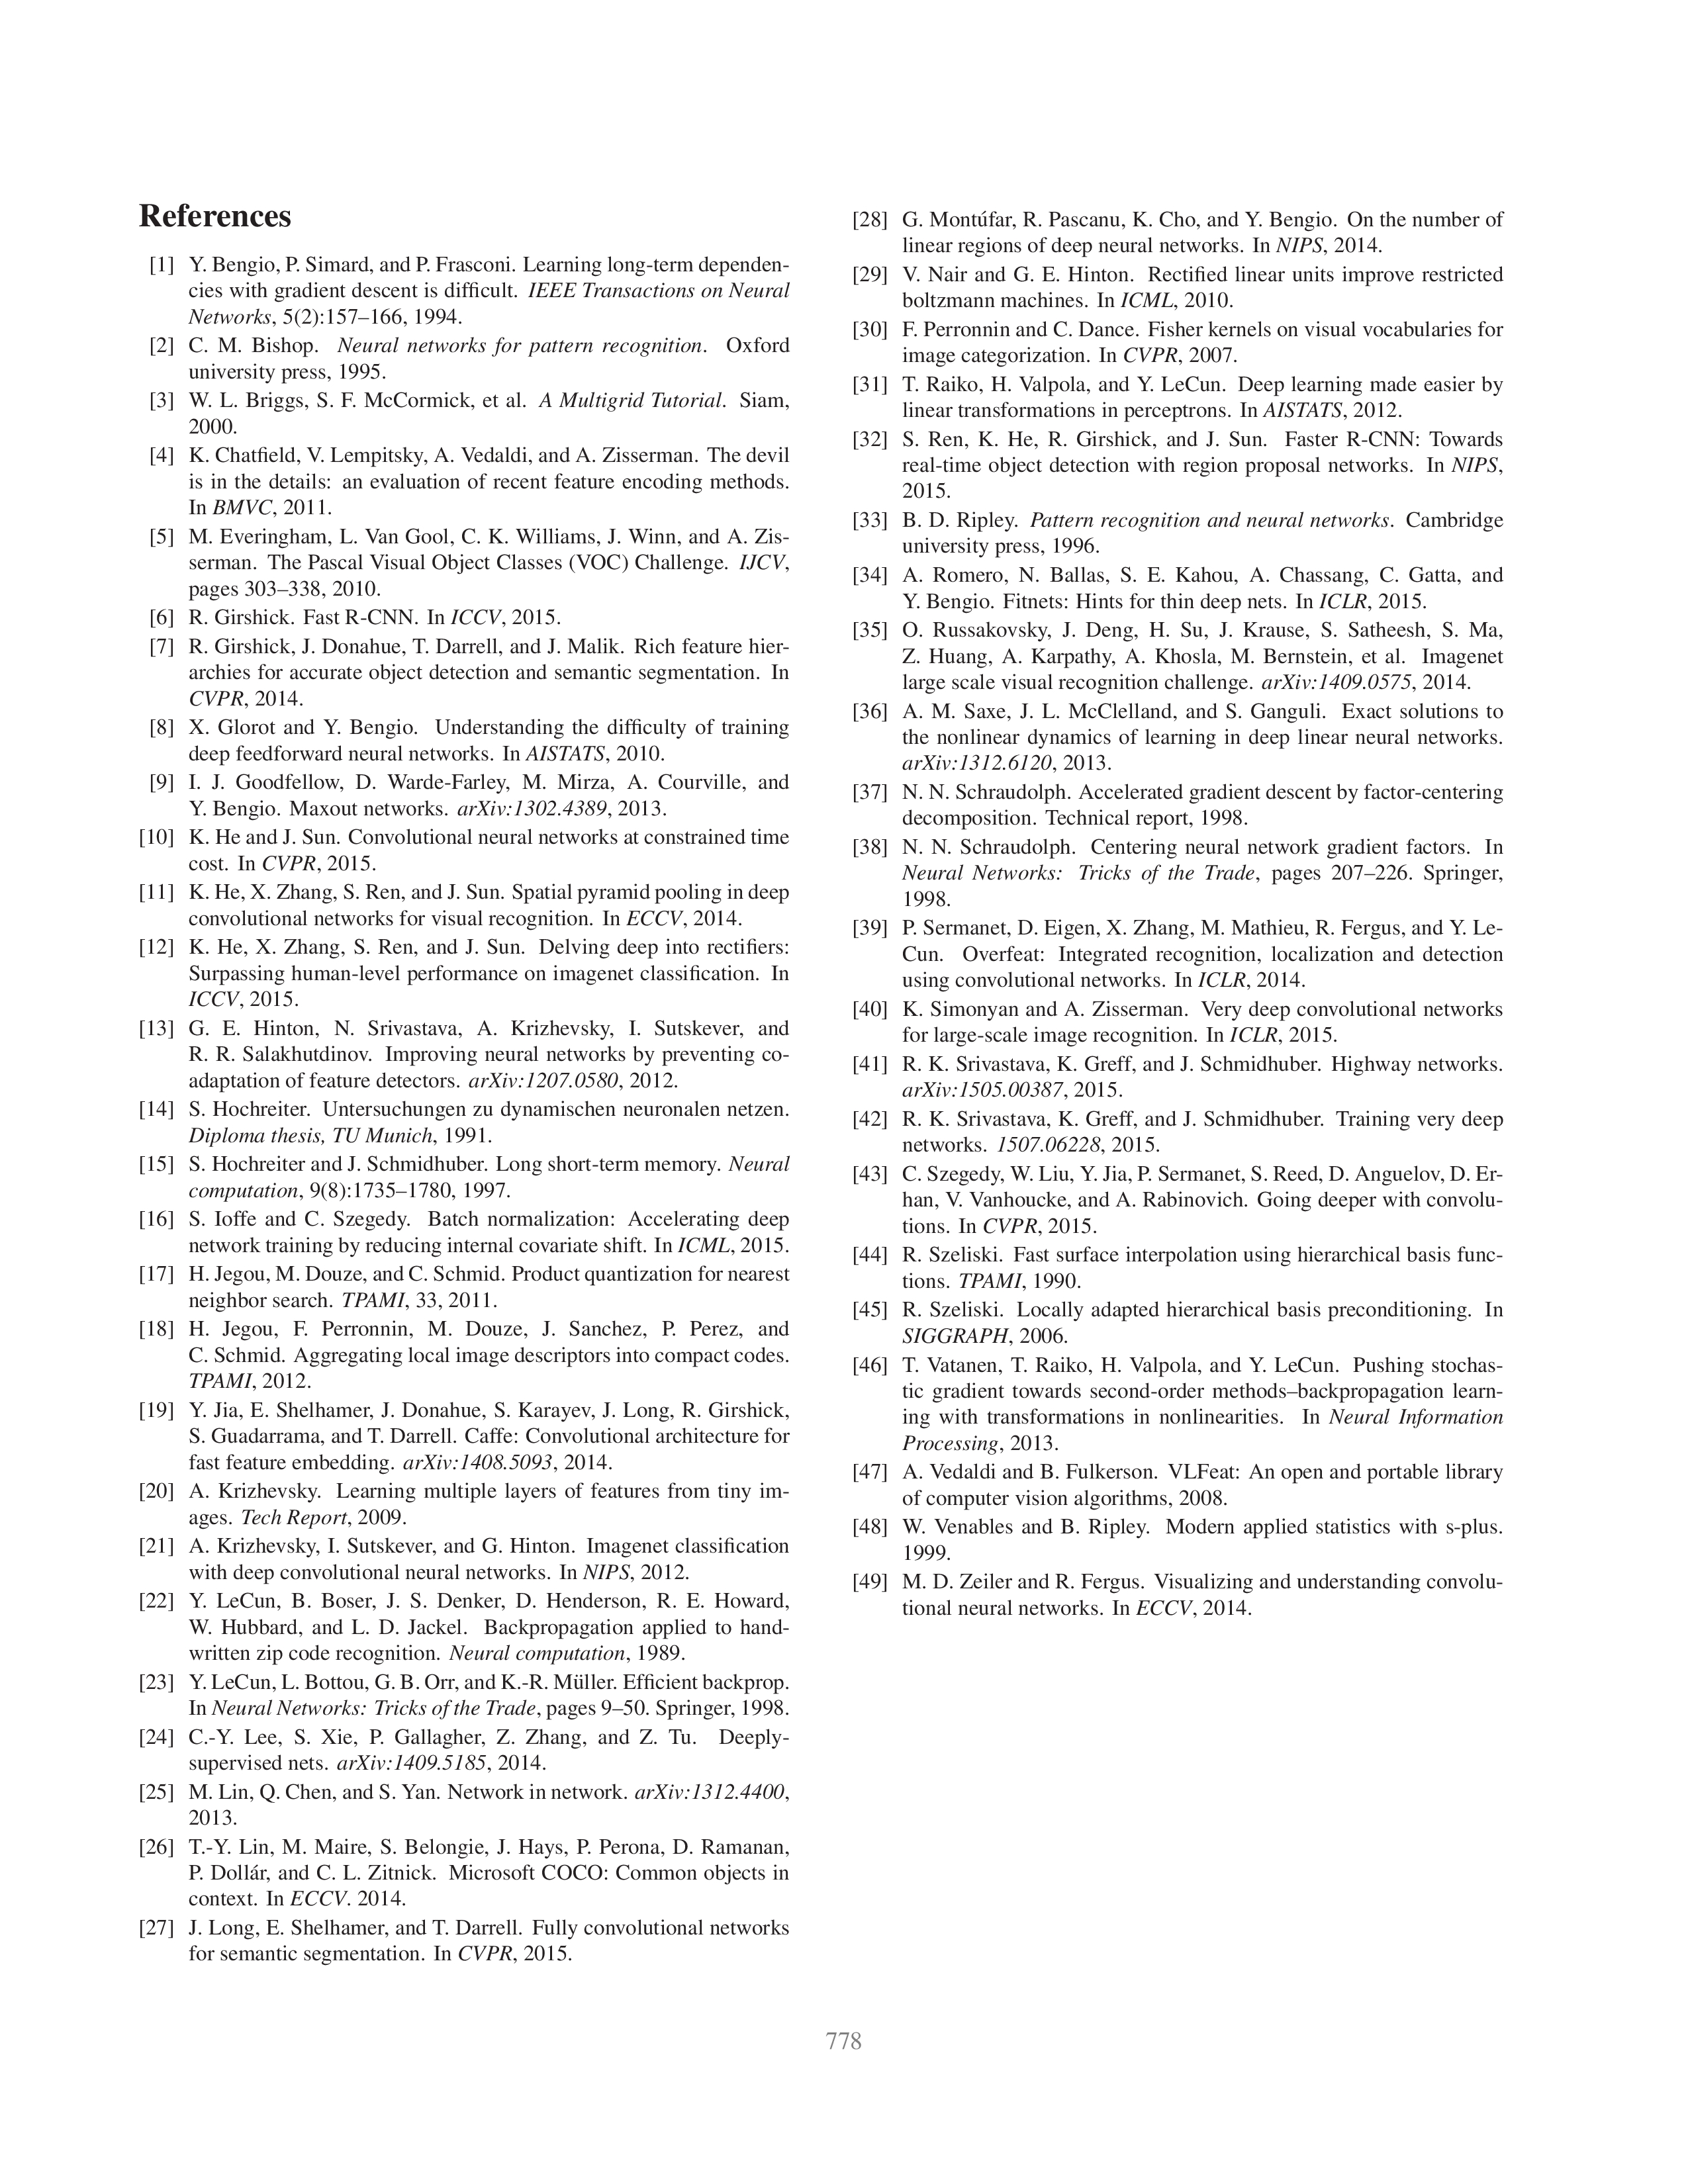
\includegraphics[width=\textwidth]{figures/english/english-8.jpg}
% \end{figure}				% 外文资料
% !Mode:: "TeX:UTF-8"

\titlecontents{chapter}[2em]{\vspace{.5\baselineskip}\xiaosan\song}
             {\prechaptername\CJKnumber{\thecontentslabel}\postchaptername\qquad}{}
             {}             % 设置该选项为空是为了不让目录中显示页码
\addcontentsline{toc}{chapter}{中文译文}
\setcounter{page}{1}            % 单独从 1 开始编页码
\markboth{中文译文}{中文译文}   % 用于将章节号添加到页眉中
\chapter*{中文译文}

\trtitle{图像识别的深层残差网络}

\trchapter{介绍}

深层残差网路对于图像分类问题已经有了很多的突破,深层网络通常会整合低\\中\\高三中不同的层特征,并将其分类到多种层方法上,由此,层特征可以通过堆叠层的数量增多而得到增强。最近的研究表明了网络的深度很重要,而最新的研究中,针对ImageNet的深层网络达到了从16层到30层。其他很多平凡的视觉检测任务也在深层模型中有很对的益处。

被网络深度的优点驱动,我们会得到一个问题:是否随着堆叠层的层数增多,其学习的效率就会越高嘛?很重要的一个问题就是梯度消失。正太分布的参数初始化和中间标准化层已经有很多显示这个问题了,其能允许有着数层的网络能够为反向传播的随机的梯度下降产生收敛的效果。

当更深的网络开始收敛时,梯度消失就暴露了出来:随着网络深度增加,准确率开始饱和,真实缓慢降低。这种降低并非是由过拟合造成的,添加更多的层会导致更大的训练误差,正如之前的成果表明的那样,我们的实验也证明了这一点。

训练准确率的降低暗示了并非所有的系统都能这么简单的去优化。让我们考虑一个更为浅层的网络结构,并且其更深层的副本会增加更多的层。我们生层深层模型时有一种结对方法:添加的层是其他层的相等映射,即其是浅层模型层的拷贝。这种方法揭示了深层模型不应该产生比浅层模型更少的训练误差。但是实验显示我们现在的解决方法并不能找到一个相比于生成方案更为合适的方法。

在这篇文章中,我们引入了深层残差学习框架,并非期望少数堆叠层能直接适应于底层映射,我们使用残差映射。我们一般的将其映射定义为 $ H(x) $,我们将堆叠的非线性层匹配于另一个映射定义为 $ F(x) = H(x) -x $ , 原来的映射被重定义为 $ F(x)+x $。我们假设相比于原来的网络,残差映射能够更好的优化。如果一个恒等映射被最优化了,则会更容易将残差优化到0。

我们的公式 $ F(x)+x $ 可以看作一个捷径链接,其会跳过一到多个层。在我们的情况下,这种捷径连接简单的使用了恒等映射技术,并且他们的输出被简单的加到了堆叠层中。恒等捷径连接并未添加了额外的参数或是额外的复杂度。整个网络仍接可以通过梯度下降训练反向传播,也能通过共同库来进行实现。

我们在ImageNet上的实验显示了梯度消失问题并验证了我们的方法,实验显示:1)我们的残差网络能够很简单地进行优化,但简单网络有更大的误差。2)我们的残差网络能够很简单通过增加深度获得准确的增益。

相似的现象也在CIFAR-10数据集上产生了,暗示了优化难度以及我们的方法并非限制于特定的数据集,我们在超过100层的数据集甚至于超越1000层的网络中有很好的训练效果。

在ImageNet分类数据集中,我们也有着很好的结果。我们的152层残差网络是已知的针对这个最深的网络了。也仍旧比VGG网络有更好的效果。在ImageNet测试集上我们有3.75\%的top5误差,并获得了ILSVRC2015的分类比赛冠军。在其他识别问题上这个也获得了很好的效果,并让我们获得了很多其他的冠军。

\trchapter{相关工作}

\trsection{残差表示}

在图像识别的领域里,VLAD是通过残差响亮编码的表示,Fisher向量能被格式化为VLAD的概率化版本。他们都是对于图像检索和分类都很有效。对于矢量量化,编码残差向量显示出比编码原始向量更有效。在低级视觉和计算机图形学中,用于求解偏微分方程被广泛使用多重网格方法,将系统重新制定为多个尺度的子问题,其中每个子问题负责较粗和较精细之间的残差解。Multigrid的替代方法是层次基础预处理,它依赖于表示两个尺度之间的残差向量的变量。这些求解器比不知道解的残余性质的标准求解器收敛得快得多。 这些方法表明良好的重构或预处理可以简化优化过程。

\trsection{捷径连接}

长期以来,人们一直在研究导致捷径连接的实践和理论。训练多层感知器(MLP)的早期实践是添加从网络输入连接到输出的线性层。 一些中间层直接连接到辅助分类器,以解决消失/爆炸梯度。 这些论文提出了通过捷径连接实现的中心层响应,渐变和传播错误的方法。 “初始”层由捷径分支和几个更深的分支组成。

与我们的工作相比,“高速公路网络”提供与门控功能的捷径连接。 与我们的无参数身份捷径方式相比,这些门是数据相关的并且具有参数。当门控捷径方式“关闭”(接近零)时,公路网络中的层表示非残差功能。 相反,我们的表述总是学习剩余的功能; 我们的恒等捷径方式永远不会关闭,所有信息都会通过,并且我们还需要学习额外的残差功能。但此外,高速网络在深度增加极大的同时并没有显着提高精度。

\trchapter{深层残差学习}

\trsection{残差学习}

让我们将$ H(x)$ 视为底层映射,使其适合几个堆叠层(不一定是整个网络),$x$表示这些层中第一层的输入。 如果假设多个非线性层可以渐近逼近复杂函数,那么它等效于假设它们可以渐近逼近残差函数,即$H(x)-x$(假设输入和输出具有相同的维度)。 因此,我们明确地让这些层近似于残差函数$F(x):= H(x) -  x$,而不是期望堆叠层接近$H(x)$。 因此原始函数变为$F(x)+ x$。 虽然两种形式都应该能够渐近地逼近所需的函数,但学习的难度可能会有所不同。

产生这种重格式化的动机是由于退化问题的反直觉的现象。正如在引言中所讨论的,如果添加的层可以构造为恒等映射,则更深的模型应该不具有比其较浅的对应物更大的训练误差。退化问题表明,求解器可能难以通过多个非线性层来近似同一性映射。利用残差学习重构,如果恒等映射是最优的,则求解器可以简单地将多个非线性层的权重推向零以接近恒等映射。

在实际情况下,恒等映射不太可能是最优的,但我们的重构可能有助于预先解决问题。如果最优函数更接近于恒等映射而不是零映射,则求解器应该更容易参考恒等映射来查找扰动,而不是将该函数作为新映射来学习。我们通过实验表明,学习的残差函数通常具有较小的响应,这表明恒等映射提供了合理的预处理。

\trsection{基于捷径的恒等映射}

我们每个堆叠层都采用残差学习。构建块如图2所示。在本文中,我们定义构建块:

\begin{eqnarray}
    y = F(x,\{W_i\})+x
    \label{euq:tran-1}
\end{eqnarray}

这里 $ x $ 和 $ y $ 是输入和输出向量。函数 $ F(x,\{W_i\}) $ 表示了要被学习的残差映射。比方说两层 $ F = W_2 \sigma ( W_1 x) $,这里 $ \sigma $ 表示了线性整流函数,我们还省略了偏置以简化符号。通过捷径连接和逐元素添加来执行操作 $ F+x $ 。在加法后我们采用第二非线性。

方程\ref{euq:tran-1}中的捷径方式连接既不引入额外参数也不引入计算复杂性。 这不仅在实践中具有吸引力,而且在我们对普通网络和剩余网络之间的比较中也很重要。 我们可以公平地比较同时具有相同数量的参数、深度、宽度和计算成本的普通/残差网络(除开可忽略的元素添加)。

公式\ref{euq:tran-1}中 $ x $ 和 $ F $ 的尺寸必须相等。 如果不是这种情况(比方说在更改输入/输出通道时),我们可以通过捷径方式连接执行线性投影$ W_s $以匹配尺寸:

\begin{eqnarray}
    y = F(x,\{W_i\}) + W_s x
    \label{euq:tran-2}
\end{eqnarray}

我们也可以在方程\ref{euq:tran-1}中使用矩阵 $W_s$。 但是我们将通过实验证明,恒等映射足以解决退化问题,并且它是经济的,因此 $W_s$一般只在匹配维度时使用。

残差函数$F$的形式是灵活的。本文中的实验涉及具有两层或三层的函数$F$,而更多层也并非不可。 但是如果$F$只有一层,则方程\ref{euq:tran-1}类似于线性层:$y = W_1x + x$,这样就没有啥优点了。

我们还注意到,尽管为简单起见,上述符号是基于全连接层,但它们也适用于卷积层。函数$F(x,\{W_i\})$可以表示多个卷积层。并两个特征映射上逐个通道执行逐元素的添加。

\trsection{网络结构}

我们测试了各种普通/残差网洛,并观察到了一致的现象。为了提供讨论的实例,我们为ImageNet描述了两个模型,如下所示。

\trsubsection{简单网络}

我们的简单网络主要受到VGG网络的启发。卷积层大多具有 $ 3\times3 $滤波器并遵循着两个简单的设计规则:(i)对于相同的输出特征映射大小,这些层具有相同数量的滤波器; (ii)如果特征映射大小减半,则过滤器的数量加倍,以便保持每层的时间复杂度。 我们直接通过步幅为2的卷积层进行下采样。网络最后以全局平均池层和带有softmax的1000路全连接层结束。且加权层的总数是34。

值得注意的是,我们的模型比VGG网络具有更少的过滤器和更低的复杂性。我们的34层简单网络有36亿FLOP(乘法增加),仅为VGG-19(196亿FLOP)的18%。

\trsubsection{残差网络}

基于上述普通网络,我们插入了捷径连接,将网络转换为对应的残差版本。 当输入和输出具有相同的尺寸时,可以直接使用标识捷径方式(公式\ref{euq:tran-1})(图3中的实线快捷方式)。 当尺寸增加时(图3中的虚线快捷键),我们考虑两个选项:(A)捷径方式仍然执行恒等映射,为增加尺寸填充额外的零条目。此选项不引入额外参数;(B)方程(2)中的投影捷径方式用于匹配尺寸(由$1\times1$卷积完成)。 对于这两个选项,当捷径方式跨越两种尺寸的特征图时,它们的步幅为2。

\trsection{实现}

我们对ImageNet的实现遵循[21,41]中的实践,我们调整图像大小,其短边在 $[256,480]$ 中随机采样用于尺度增强[41]。从图像或其水平翻转中随机进行 $224\times224$ 裁剪采样,减去每像素平均值[21]。使用[21]中的标准颜色增强。 我们在每次卷积之后和激活之前采用批量归一化(BN)[16]。再之后,我们在[13]中初始化权重,并从头开始训练所有普通/残差网洛。我们使用小批量256的SGD。学习率从0.1开始,当误差平稳时再除以10,并且模型训练最多$60\times10^4$次迭代。我们使用$0.0001$的衰减系数和$0.9$的动量系数。按照[16]中的实践,我们不使用dropout[14]。

在测试时,出于比较研究,我们采用标准的10种作物测试[21]。为了获得最佳结果,我们采用[41,13]中的全卷积形式,并在多个尺度上平均获得得分(图像被调整大小,使得短边在$\{224; 256; 384; 480; 640\}$ 之中)。

\trchapter{实验结果}

\trsection{ImageNet分类}

我们在由1000个类组成的ImageNet-2012分类数据集上评估我们的方法。模型在128万个训练图像上进行训练,并在50k验证图像上进行评估。我们还获得了测试服务器报告的100k测试图像的最终结果。我们评估top-1和top-5的错误率。

\trsubsection{简单网络}

我们首先评估18层和34层简单网。34层普通网在图3(中间)。18层普通网具有类似的形式。

表2中的结果表明,较深的34层简单网络比较浅的18层简单网络具有更高的验证误差。为了揭示其中原因,在图4(左)中我们比较了他们在训练过程中的训练/验证错误。我们观察到了退化问题——即使18层简单网络的解空间是34层简单网络的子空间,34层普通网在整个训练过程中也有较高的训练误差。

我们认为这种优化难度不太可能是由于梯度消失造成的。这些普通网络采用BN[16]进行训练,确保前向传播信号具有非零方差。我们还验证了向后传播的梯度与BN表现正常。因此,前向和后向信号都不会消失。事实上,34层普通网仍然能够达到有竞争力的准确度(表3),这表明求解器在某种程度上起作用。 我们推测深层简单网可能具有指数级的低收敛速度,这会影响训练误差的减少。将来将研究这种优化困难的原因。

\trsubsection{残差网络}

我们评估了18层和34层残差网洛(ResNets)。基础架构与上述简单网络相同,期望在每对 $3 \times 3$滤波器中添加快捷连接,如图3(右)所示。 在第一次比较中(表2和图4右),我们对所有捷径方式使用恒等映射,为增加维度使用零填充(选项A)。 因此,与普通同行相比,他们也没有额外的参数。

我们从表2和图4中得到了三个主要观察结果。首先,情况与残差学习相反——34层ResNet优于18层ResNet(2.8%)。更重要的是,34层ResNet表现出相当低的训练误差,并且可以推广到验证数据。 这表明在该设置中很好地解决了退化问题,并且我们设法从增加的深度获得准确性上的增益。

其次,与普通对应物相比,由于成功减少了训练误差(图4右对左),34层的ResNet将前1个误差减少了3.5%(表2)。该比较验证了极深系统上残差学习的有效性。

最后,我们还注意到18层简单/残留网络是相对准确的(表2),但18层ResNet收敛速度更快(图4右侧与左侧)。当网络“不太深”(此处为18层)时,当前的SGD求解器仍然能够找到简单网络的良好解决方案。 在这种情况下,ResNet通过在早期阶段提供更快的收敛来简化优化。

\trsubsection{恒等和投影的比较}

我们已经证明,无参数的恒等捷径方式有助于训练。接下来我们研究投影捷径方式(方程(2))。 在表3中,我们比较了三个选项:(A)零填充快捷方式用于增加尺寸,所有捷径方式都是无参数(与表2和图4相同); (B)投影快捷方式用于增加尺寸,其他快捷方式是标识; (C)所有捷径都是预测。

表3显示所有三个选项都明显优于简单网络对应选项。B稍微好于A.我们认为这是因为A中的零填充维度确实没有残差学习。C略微优于B,我们将其归因于许多(13个)投影捷径方式引入的额外参数。但A/B/C之间的微小差异表明,预测捷径对解决退化问题并不重要。因此,我们在本文的其余部分不使用选项C来减少内存/时间复杂度和模型大小。恒等捷径方式对于不增加瓶颈架构的复杂性特别重要。
				% 中文译文
% % !Mode:: "TeX:UTF-8"

\titlecontents{chapter}[2em]{\vspace{.5\baselineskip}\xiaosan\song}
             {\prechaptername\CJKnumber{\thecontentslabel}\postchaptername\qquad}{} 
             {}                            % 设置该选项为空是为了不让目录中显示页码
\fancypagestyle{plain}{
    \fancyhf{}
    \fancyhead[C]{\song\wuhao 天津大学 2015 届本科生毕业论文}
}           

\markboth{致\qquad 谢}{致\qquad 谢}
\addcontentsline{toc}{chapter}{致谢} % 添加到目录中
\chapter*{致\qquad 谢}

本论文的完成我衷心的感谢指导老师陈瑞教授,是在他的指导下让我对这几年看的东西进行了梳理和总结,在论文写作期间,加深了对很多原理和知识的理解,也由此对现在的前沿技术有所涉猎。

此外,希望这论文能是我的启航线吧。				% 致谢	
\clearpage 
\end{document}									% 结束全文
